\clearpage
\setcounter{figure}{8}
\setcounter{table}{1}
\crshead{ГЛАВА 3. Практический анализ и сравнение источников энтропии}

\crssubhead{3.1. Сравнительный анализ источников энтропии}

Сравнение различных физических и квантовых источников энтропии
показывает, что каждый из них обладает уникальными преимуществами и
ограничениями, что делает их пригодными для разных сфер применения в
зависимости от конкретных требований к качеству случайности, уровню
безопасности, потребляемым ресурсам и технологическим возможностям
интеграции.

Физические источники энтропии, такие как тепловой шум, дробовой шум,
лавинный шум и мерцающий шум, характеризуются относительно простой
схемотехнической реализацией и возможностью интеграции в существующие
полупроводниковые платформы. Это делает их особенно привлекательными для
встраивания в микроконтроллеры, криптографические процессоры и другие
устройства массового производства. Однако такие источники могут быть
чувствительны к температурным колебаниям, электромагнитным наводкам,
старению компонентов и другим нежелательным факторам, которые могут
вносить детерминированные искажении в сигнал, снижая истинную энтропию.
Например, тепловой шум достаточно стабилен, но имеет сравнительно низкую
энтропийную мощность, что ограничивает его скорость генерации. Дробовой
и лавинный шумы более насыщены энтропией и менее предсказуемы, но
требуют сложной схемы усиления и фильтрации, а также могут генерировать
импульсные сигналы, неравномерные по амплитуде и длительности. Мерцающий
шум отличается высокой интенсивностью при низких частотах, но сложен для
оценки и контроля, а также может быть подвержен воздействию окружающей
среды.

Квантовые источники энтропии, основанные на таких явлениях, как
квантовые переходы, туннелирование, спонтанное излучение или рассеяние
фотонов, обеспечивают наивысший уровень истинной случайности, поскольку
происхождение сигнала невозможно описать детерминированными законами
физики. Это делает такие источники предпочтительными для задач, где
требуется абсолютная непредсказуемость, например, в генерации ключей для
квантово-устойчивой криптографии. Однако их реализация требует
прецизионной оптики, фотонных детекторов, лазеров или других сложных
квантово-оптических компонентов. Это не только увеличивает стоимость
устройств, но и требует особых условий эксплуатации, включая защиту от
вибраций, температурную стабилизацию и экранирование от внешних
воздействий. Кроме того, из-за высокой чувствительности к шумам и дрейфу
параметров оборудования, такие системы нуждаются в регулярной калибровке
и контроле качества работы.

Макроскопические и хаотические источники энтропии основаны на трудно
моделируемых динамических процессах, таких как движение в турбулентных
потоках, случайные колебания в нелинейных цепях или шум в радиоэфире.
Они интересны прежде всего своей простотой в реализации и возможностью
достигать очень высокой скорости генерации, что особенно полезно для
приложений, не связанных с криптографией, но требующих большого
количества случайных данных (например, в компьютерных играх или
симуляционных моделях). Однако эти источники страдают от высокой
зависимости от внешних условий и трудно поддаются строгой математической
верификации, что делает их менее надёжными в задачах, где требуется
доказуемо высокая энтропия. Кроме того, при известной модели системы, в
теории, возможно частичное предсказание поведения хаотического
источника, особенно если используется псевдослучайный усилитель
динамики.

В обобщении, можно сказать, что физические источники --- это компромисс
между простотой, скоростью и надёжностью, квантовые --- максимум
безопасности и непредсказуемости при высокой стоимости, а хаотические ---
высокая производительность при умеренном уровне доверия. Поэтому выбор
зависит от того, что критично в конкретной системе: высокая скорость,
минимальные затраты, интегрируемость или гарантированная случайность.

\crssubhead{3.2. Архитектура экспериментального стенда и программная инфраструктура}

Практическая часть работы построена вокруг компактного измерительного стенда на базе
платы Arduino Nano с микроконтроллером ATmega328P и набора прикладных программ для
персонального компьютера. Принятый подход --- последовательная унификация: для каждого
исследуемого физического канала энтропии создаётся отдельная прошивка и собственная
аналоговая обвязка, однако формат отсчётов, конвейер постобработки и пакет статистических
процедур одинаковы для всех источников. Такая организация позволяет, во-первых,
сопоставлять источники между собой при идентичных условиях регистрации, и, во-вторых,
добавлять новые экспериментальные каналы без переделки общей инфраструктуры
измерений и анализа.

\crssubhead{3.2.1. Назначение и модульная организация}

Стенд решает четыре последовательные задачи: регистрацию потоков отсчётов
аналого-цифрового преобразователя (АЦП), сохранение этих потоков в виде воспроизводимых
двоичных массивов, преобразование выборок в битовые последовательности при помощи
постобработки и, наконец, количественную оценку случайности полученных потоков ---
вплоть до запуска эталонного пакета NIST Statistical Test Suite. В архитектурном плане
выделяются пять логически независимых уровней: измерительный узел на микроконтроллере
с первичным датчиком; двоичный протокол передачи данных по последовательному
каналу USB-CDC; программы захвата и сохранения метаданных сеанса на хост-компьютере;
блок численного анализа и автоматического формирования отчётов; и уровень формальной
верификации случайности по методике NIST STS. Схемные решения и перечень элементов
для каждого канала приводятся непосредственно в соответствующих разделах настоящей
главы и поставлены в соответствие с теоретическими разделами главы~2.

\crssubhead{3.2.2. Аппаратная база и прошивки микроконтроллера}

Измерительным узлом служит плата Arduino Nano с микроконтроллером ATmega328P,
имеющим встроенный десятиразрядный АЦП последовательного приближения и аппаратный
интерфейс UART, выведенный через мост USB--UART на разъём USB-C хост-компьютера.
Аналоговые источники энтропии подключаются к входам АЦП (как правило, к каналу A0);
цифровые датчики --- к шине I$^2$C с программной упаковкой считанных регистров в
единый формат шестнадцатибитных слов, совместимый со всеми остальными каналами стенда.

Реализованный набор каналов охватывает: тепловой шум прецизионного резистора
(глава~2.1), лавинно-дробовой режим обратносмещённого перехода биполярного транзистора,
акустический модуль на электретном капсюле, MEMS-инерциальный датчик MPU-6050,
режим <<плавающего>> входа АЦП для учёта электромагнитных наводок, оценку дрожания
тактов относительно сторожевого таймера (clock jitter), а также гибридную комбинацию
нескольких независимых каналов с последующим смешением на стороне ПК (постобработка
XOR + SHA-256).

Для каждого канала разработан отдельный скетч прошивки. Общие элементы --- бинарный
последовательный протокол и процедура ускоренной выборки АЦП в режиме свободного
запуска (\textit{free-running}, прескалер $16 \Rightarrow$ частота преобразования АЦП
$\approx 76{,}9$~кГц) --- вынесены в разделяемые заголовочные файлы и подключаются
всеми конфигурациями. При программировании контроллера задаются символьный
идентификатор источника, номинальная частота преобразования АЦП, разрядность полезной
части АЦП при выбранном опорном напряжении и поясняющая строка о навесных элементах;
эти поля автоматически попадают в метаданные сеанса записи. Важно различать
\emph{частоту преобразования} АЦП (с которой работает свободный запуск) и
\emph{фактическую частоту отсчётов} записанного потока: как показано в разделе~3.2.3,
последняя определяется пропускной способностью канала связи и оказывается заметно
ниже.

\crssubhead{3.2.3. Бинарный протокол обмена и захват данных}

После сброса микроконтроллер передаёт по USB-CDC короткий ASCII-баннер служебных строк,
сообщающих формат двоичной фазы (\textit{little-endian}, беззнаковые 16-битные слова),
номинальную частоту опроса АЦП, тип опорного напряжения и комментарий о навесной обвязке.
За маркером начала двоичной части следует непрерывный поток двухбайтовых слов без
разбиения на пакеты фиксированной длины. Скорость линии последовательного интерфейса
устанавливается равной $10^6$~бод. Вопреки распространённому представлению об
<<ограничении COM-порта в $115\,200$~бод>>, эта величина не является пределом:
Arduino Nano подключается через USB-мост (CH340 / FT232), а не через физический порт
RS-232, а для тактовой частоты $16$~МГц именно $10^6$~бод даёт \emph{нулевую} ошибку
делителя UART (тогда как у $115\,200$~бод при $16$~МГц ошибка составляет ${\approx}3{,}5\%$).

Именно последовательная линия, а не АЦП, оказывается узким местом измерительного
тракта. При кадре $8\text{N}1$ ($10$ бит на байт) канал $10^6$~бод переносит
$10^6/10 = 100\,000$~Б/с, то есть $50\,000$ двухбайтовых отсчётов в секунду.
Поскольку основной цикл прошивки блокируется на отправке каждого слова в
последовательный порт, частота записанного потока ограничивается сверху этим
значением: измеренная по объёму файла и длительности сеанса фактическая частота
отсчётов электронных каналов составляет $f_s\approx 49{,}6$~кГц --- вплотную к
теоретическому потолку линии и существенно ниже частоты преобразования АЦП
($76{,}9$~кГц). <<Лишние>> преобразования свободного запуска при этом просто не
передаются (отправляется последнее готовое). Для каналов с пониженной частотой
преобразования (например, акустического, $38{,}5$~кГц) поток укладывается в
пропускную способность линии, и фактическая частота отсчётов совпадает с
номинальной.

На стороне ПК соответствующий скрипт (\texttt{capture/capture\_serial.py}) принимает
поток из устройства последовательного порта, отделяет ASCII-преамбулу от двоичной части,
сохраняет последнюю как массив отсчётов фиксированного формата и сериализует
метаданные сеанса в JSON-файл рядом с дампом. Это обеспечивает воспроизводимость
эксперимента: длительность записи рассчитывается из числа байт и временных меток
приёмника, а параметры АЦП восстанавливаются из преамбулы автоматически.

\crssubhead{3.2.4. Конвейер обработки на персональном компьютере}

Из массива отсчётов первой операцией извлекаются выбранные младшие двоичные разряды
(\textit{least significant bits}, МЗР) каждого слова --- получается упакованный битовый
файл. Опционально к нему применяется постобработка по схеме фон Неймана (\textit{von
Neumann debiasing}), устраняющая статистическое смещение в предположении независимости
пар бит. Дополнительно поддерживаются альтернативные процедуры (XOR-децимация,
криптографическое отбеливание SHA-256), сравнительные результаты которых также
учитываются при анализе.

Отдельные программные модули вычисляют гистограмму распределения уровней (с тестом
$\chi^2$ на равномерность), оценивают спектральную плотность мощности методом Уэлча,
строят нормированную автокорреляционную функцию выборок и битов, рассчитывают
энтропию на символ (Шеннон, минимальная энтропия по NIST SP~800-90B) и формируют
растровое изображение фрагмента битового потока заданного размера для визуальной оценки
структурных артефактов. Объединяющий конвейерный сценарий (\texttt{scripts/pipeline.py})
последовательно запускает захват, постобработку, статистические тесты и сборку
итогового отчёта; это исключает рассогласование версий данных между этапами и
снижает риск ошибок ручного запуска.

\crssubhead{3.2.5. Интеграция с NIST STS}

Для формализованной верификации двоичных последовательностей подключается оригинальная
реализация NIST STS версии $2{,}1{,}2$. Подготовленные битовые файлы подаются на вход
утилиты \texttt{assess}; стандартный режим работы --- десять независимых битовых потоков
по $10^6$ бит каждый. Сырой выходной отчёт \texttt{finalAnalysisReport.txt} парсится
скриптом-агрегатором в компактное представление: для каждой группы тестов фиксируются
число подтестов, минимальное и максимальное сводное $p$-значение, доля прошедших
подтестов и итоговый групповой вердикт PASS / FAIL / N/A. Эта ступень дополняет
теоретический материал главы~1 практической иллюстрацией: расхождения между
вердиктами для <<сырых>> бит и для последовательности после фон Неймана, появление
статуса <<неприменимо>> у тестов RandomExcursions и RandomExcursionsVariant при
выраженном смещении --- всё это свойства данных и области применимости конкретных
критериев пакета, а не ошибка связки аппаратуры с программами.

\crssubhead{3.3. Аналоговый усилительный тракт}

Большинство рассматриваемых в работе физических источников шума (тепловой шум
резистора, лавинно-дробовой шум обратносмещённого перехода BJT) даёт на выходе
напряжение порядка единиц или десятков микровольт, что лежит ниже разрешения АЦП
ATmega328P (около $4{,}9$~мВ на младший разряд при $U_\mathrm{REF}=5$~В). Поэтому
между датчиком шума и аналоговым входом микроконтроллера обязательно присутствует
усилительный тракт с коэффициентом усиления от $10^2$ до $10^4$. В данной работе
использованы две топологии: одно- и двухкаскадный неинвертирующий усилитель на базе
доступных дешёвых операционных усилителей (ОУ).

\crssubhead{3.3.1. Выбор операционного усилителя}

Эксперименты проводились с двумя ОУ --- LM358N и TL072CP. Их выбор обусловлен
типовой доступностью в любительских условиях, наличием двух идентичных каналов в одном
корпусе DIP-8 (удобно для двухкаскадной схемы) и работой от одиночного напряжения
питания $+5$~В (LM358) или биполярного питания (TL072). Основные характеристики,
существенные для задачи усиления широкополосного шума малой амплитуды, сведены в
таблице~\ref{tab:opamp_compare}.

\begin{table}[H]
  \centering
  \footnotesize
  \caption{Сравнение характеристик операционных усилителей LM358 и TL072, использованных в стенде}
  \label{tab:opamp_compare}
  \begin{tabular}{|p{0.30\linewidth}|p{0.30\linewidth}|p{0.30\linewidth}|}
    \hline
    Параметр & LM358 (bipolar) & TL072 (JFET-input) \\
    \hline
    Тип входного каскада & биполярный (BJT) & полевой (JFET) \\
    \hline
    Напряжённая плотность шума на входе $e_n$ при $1$~кГц & ${\approx}40$~нВ/$\sqrt{\mathrm{Гц}}$ & ${\approx}18$~нВ/$\sqrt{\mathrm{Гц}}$ \\
    \hline
    Токовая плотность шума на входе $i_n$ & ${\approx}0{,}5$~пА/$\sqrt{\mathrm{Гц}}$ & ${\approx}0{,}01$~пА/$\sqrt{\mathrm{Гц}}$ \\
    \hline
    Произведение усиление-полоса (GBW) & $1{,}0$~МГц & $3{,}0$~МГц \\
    \hline
    Максимальное напряжение выхода (rail-to-rail) & до $U_{CC}-1{,}5$~В (нижнего рельса касается) & ограниченная $\pm U_{CC}$, требует биполярного питания \\
    \hline
    Питание & $+3{\ldots}+32$~В однополярное & $\pm 4{,}5{\ldots}\pm 18$~В биполярное \\
    \hline
  \end{tabular}
\end{table}

Принципиально важная для данной задачи особенность LM358 состоит в том, что выход
этого ОУ способен подходить вплотную к нижнему рельсу питания (${\sim} 0{,}1$~В),
однако не достигает верхнего --- его динамический диапазон ограничен сверху
значением $U_{CC}-1{,}5$~В. При питании $+5$~В это означает практический потолок
выхода ${\approx} 3{,}5$~В, что напрямую отражается на форме регистрируемого
сигнала и впоследствии (раздел~3.5) вынудило выбрать опорное напряжение делителя
$V_\mathrm{mid}$ ниже стандартного.

TL072, в свою очередь, имеет почти на порядок меньшую токовую плотность шума, что
снижает вклад больших резисторов в цепи обратной связи в общий шум тракта, и втрое
большее произведение усиление--полоса. Однако однополярное питание для TL072 не
предусмотрено: при работе только от $+5$~В реальные выходы оказываются заметно
суженным симметричным окном вокруг середины. В наших опытах с тепловым шумом
резистора (раздел~3.4) переход с LM358 на TL072 при тех же расчётных коэффициентах
усиления приводил к значительному <<сжатию>> наблюдаемого сигнала.

\crssubhead{3.3.2. Однокаскадный неинвертирующий усилитель}

Простейшая топология (рисунок~\ref{fig:amp_1stage}) представляет собой
неинвертирующий усилитель: источник шума через входной согласующий резистор
$R_\mathrm{in}$ (на схеме $R_8=100$~кОм) подаётся на неинвертирующий вход~$+$ ОУ;
отрицательная обратная связь формируется делителем $R_f/R_g$, отнесённым к
опорному напряжению $V_\mathrm{mid}$ от внешнего резистивного делителя
питания (см.~раздел~3.3.4). Коэффициент усиления по напряжению в
полосе переменного тока:
\begin{equation}
  G = 1+\dfrac{R_f}{R_g}.
  \label{eq:gain_single}
\end{equation}
Базовый набор номиналов, отражённый на схеме (рисунок~\ref{fig:amp_1stage}),
$R_g=10$~кОм ($R_5$), $R_f=470$~кОм ($R_3$); при этом $G\approx 48$. Этот
коэффициент усиления уже достаточен, чтобы лавинный шум BE-перехода BJT
становился различимым младшими разрядами 10-битного АЦП Arduino. Конкретные
значения резисторов в опытах главы~3 подбирались под уровень сигнала каждого
исследуемого источника и могут отличаться от базовых; приведённые на схеме
номиналы используются исключительно как наглядный пример.

\begin{figure}[H]
  \centering
  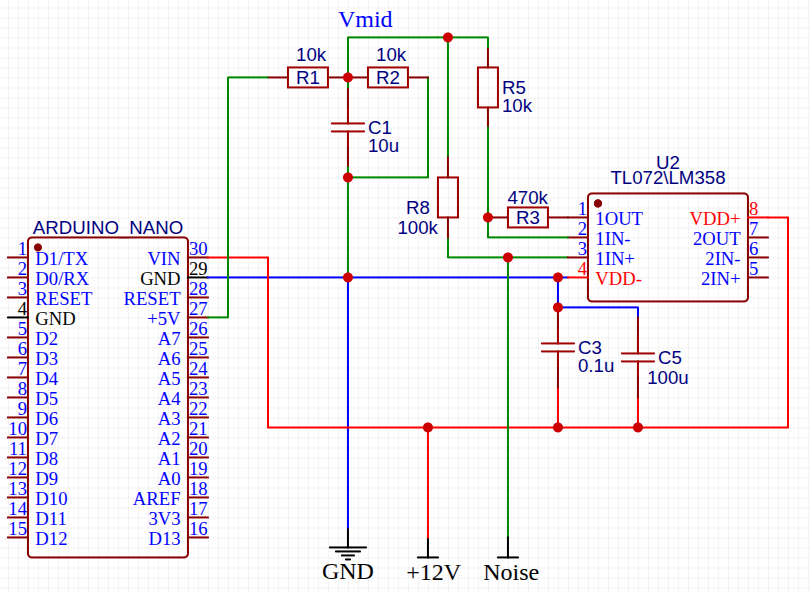
\includegraphics[width=0.95\linewidth,keepaspectratio]{pandoc_media/media/amplifier_schemas/amp_1stage.png}
  \caption{Принципиальная схема однокаскадного неинвертирующего усилителя на
  ОУ LM358 / TL072 при однополярном питании $+12$~В: $R_1,R_2$ образуют
  делитель опоры $V_\mathrm{mid}$, $C_1=10$~мкФ --- развязка опоры,
  $R_5=R_g$ и $R_3=R_f$ --- цепь обратной связи, $R_8=100$~кОм ---
  входной согласующий резистор; $C_3=0{,}1$~мкФ и $C_5=100$~мкФ ---
  развязка по питанию. Выход $1\text{OUT}$ подаётся на вход АЦП A0 Arduino Nano}
  \label{fig:amp_1stage}
\end{figure}

\clearpage
\crssubhead{3.3.3. Двухкаскадный неинвертирующий усилитель}

Если требуемое усиление превышает несколько сотен, на одиночном каскаде его
реализовать затруднительно: на больших $R_f$ растут вклад собственных шумов
резистора обратной связи, токов смещения ОУ и риск самовозбуждения тракта.
Решение --- каскадирование двух неинвертирующих усилителей. Применённая в
работе схема (рисунок~\ref{fig:amp_2stage}) использует \emph{резистивную}
связь между ступенями: выход первого каскада $1\text{OUT}$ через
последовательный резистор $R_\mathrm{c}$ (на схеме $R_4=10$~кОм; на практике
$10\ldots 100$~кОм) подаётся на инвертирующий вход второго каскада
$2\text{IN}{-}$. Такое решение, в отличие от классической AC-связи через
разделительный конденсатор, не вносит дополнительного полюса фильтра высоких
частот и сохраняет передачу низкочастотных компонент полезного сигнала, что
существенно для источников с заметным $1/f$-вкладом.

Результирующий коэффициент усиления равен произведению коэффициентов отдельных
каскадов:
\begin{equation}
  G_\Sigma = G_1\cdot G_2
           = \left(1+\dfrac{R_{f1}}{R_{g1}}\right)
             \cdot
             \left(1+\dfrac{R_{f2}}{R_{g2}}\right).
  \label{eq:gain_two}
\end{equation}

Базовый набор номиналов схемы рисунка~\ref{fig:amp_2stage}: $R_{g1}=10$~кОм
($R_5$), $R_{f1}=470$~кОм ($R_3$) даёт $G_1\approx 48$; $R_{g2}=R_4=10$~кОм,
$R_{f2}=100$~кОм ($R_6$) даёт $G_2\approx 11$, итого $G_\Sigma\approx 528$.
Конкретные значения номиналов подбирались под уровень сигнала каждого источника
и в реальных опытах могут отличаться от базовых; приведённые на схеме значения
служат иллюстративным примером. Дополнительный резистор $R_7=100$~кОм соединяет
неинвертирующий вход второго каскада $2\text{IN}{+}$ (пин~5) с шиной
$V_\mathrm{mid}$ и задаёт смещение рабочей точки второго каскада при
однополярном питании; высокое сопротивление $R_7$ выбрано так, чтобы не
шунтировать выход делителя по переменному току.

\begin{figure}[H]
  \centering
  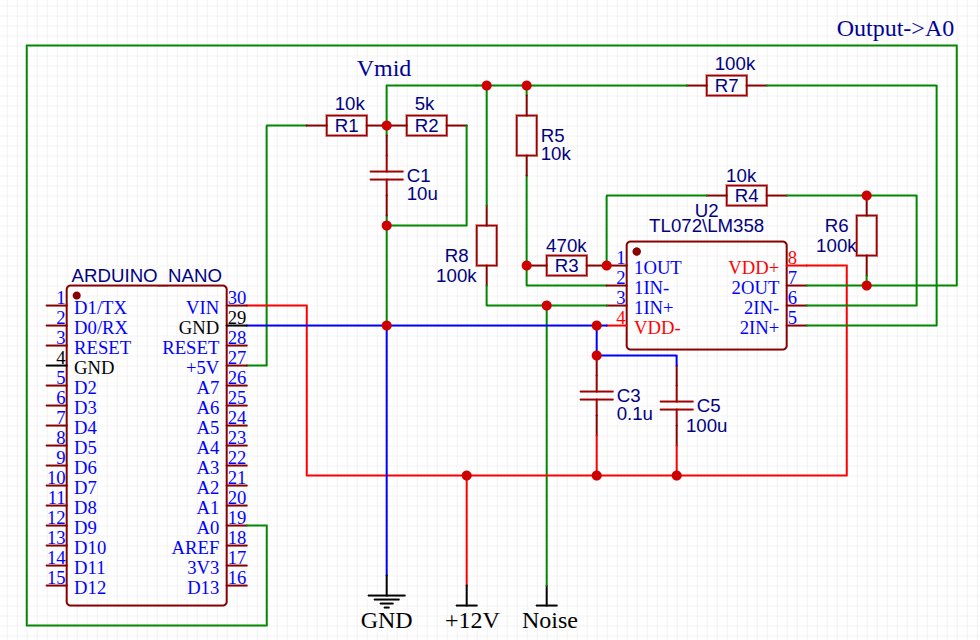
\includegraphics[width=0.97\linewidth,keepaspectratio]{pandoc_media/media/amplifier_schemas/amp_2stage.png}
  \caption{Принципиальная схема двухкаскадного неинвертирующего усилителя на
  сдвоенном ОУ LM358 / TL072 при однополярном питании $+12$~В: $R_1,R_2$ ---
  делитель $V_\mathrm{mid}$ (на схеме $R_2=5$~кОм, что соответствует
  скорректированному значению из раздела~3.5.4; в исходной конфигурации
  $R_2=10$~кОм); $R_5,R_3$ --- цепь обратной связи первого каскада;
  $R_4$ --- резистивная связь между каскадами; $R_6$ --- обратная связь
  второго каскада; $R_7$ --- резистор смещения неинвертирующего входа
  $2\text{IN}{+}$ (пин~5) к шине $V_\mathrm{mid}$. Выход $2\text{OUT}$
  подаётся напрямую на вход АЦП A0 Arduino Nano}
  \label{fig:amp_2stage}
\end{figure}

\crssubhead{3.3.4. Питание и опорное напряжение делителя}

Операционные усилители обоих каскадов запитаны от \emph{однополярного} напряжения
$+12$~В (пин $\text{VDD}{+}$ корпуса ОУ соединён с шиной $+12$~В, пин
$\text{VDD}{-}$ --- с общим проводом). Источник $+12$~В --- внешний (батарея
<<Крона>> или лабораторный блок питания); общая земля всего стенда объединяет
землю $+12$~В, землю Arduino и землю источника шума (для канала BJT ---
балластной цепи лавинного пробоя). Применение $+12$~В вместо штатных $+5$~В
Arduino обусловлено тем, что для устойчивого режима лавинного пробоя BE-перехода
BJT (раздел~3.5) необходимо напряжение, превышающее пробойное (типично
$U_{BR}\gtrsim 7\ldots 9$~В), и единая шина $+12$~В одновременно решает обе
задачи --- запитывает источник шума и усилительный тракт.

Опорное напряжение $V_\mathrm{mid}$ (его также называют <<виртуальной серединой>>
в литературе по проектированию однополярных аналоговых трактов) формируется
отдельным резистивным делителем $R_1,R_2$ (базовые номиналы $10$~кОм каждый),
подключённым между \emph{шиной $+5$~В Arduino} (выход стабилизатора платы, пин
$\text{+5V}$) и общим проводом, и шунтируется электролитическим конденсатором
$C_1=10$~мкФ для подавления пульсаций. Такое разделение питающих шин (ОУ от
$+12$~В, делитель от $+5$~В) позволяет одновременно обеспечить достаточный
диапазон вверх для выхода ОУ и удержать рабочую точку выхода в пределах
$0\ldots 5$~В входного диапазона АЦП Arduino. Полученное напряжение $V_\mathrm{mid}$
подаётся на неинвертирующий вход первого каскада (вход~$+$) и используется в
качестве <<нижнего плеча>> обратной связи первого каскада. Электролит
$C_1=10$~мкФ играет двоякую роль --- стабилизирует напряжение делителя против
пульсаций питания и снижает его выходное сопротивление в звуковой и
инфразвуковой полосе.

Дополнительно у выводов питания корпуса ОУ устанавливаются керамический
конденсатор $C_3=0{,}1$~мкФ и электролитический $C_5=100$~мкФ для подавления
высокочастотных выбросов и предотвращения паразитной генерации при большом
усилении.

\crssubhead{3.3.5. Замечание о rail-to-rail и обоснование смещения $V_\mathrm{mid}$ вниз}

Однополярное питание ОУ от $+12$~В неизбежно вводит ограничения на размах
выходного сигнала с обоих концов диапазона. Для LM358 типичное нижнее ограничение
выхода составляет $\sim 0{,}1$~В над землёй (нижний рельс достигается практически
вплотную), верхнее --- около $U_{CC}-1{,}5$~В, т.\,е.\ ${\approx}10{,}5$~В. Для
TL072 ограничение есть с \emph{обоих} концов: при $U_{CC}=+12$~В нижний предел
выхода поднимается до значения порядка $+1{,}5\ldots 2{,}0$~В (TL072 в принципе
не способен достичь отрицательного рельса даже при двуполярном питании, а в
однополярном включении от $+12$~В этот <<невидимый зазор>> сверху и снизу
оказывается заметным). Именно это ограничение --- неустранимое и пропорциональное
напряжению питания --- стало основной причиной отказа от TL072 в подавляющем
большинстве проведённых опытов: при отклонении полезного сигнала вниз от
рабочей точки амплитуда систематически срезалась границей выходного каскада,
что искажало симметрию гистограммы и вносило детерминированный артефакт в МЗР.

Кроме того, аналоговый вход АЦП Arduino принимает напряжение в диапазоне $0\ldots
U_\mathrm{REF}\approx 5$~В; всё, что превышает этот предел, ограничивается
встроенными защитными диодами и оцифровывается как насыщенное значение $1023$
(в случае выхода выше) или $0$ (ниже). При <<стандартном>> $V_\mathrm{mid}=2{,}5$~В
(делитель $R_1{=}R_2{=}10$~кОм от шины $+5$~В) рабочая точка выхода
двухкаскадного усилителя теоретически попадает ровно в центр диапазона АЦП и
оставляет симметричное окно $\pm 2{,}5$~В. Однако на практике сигнал
лавинного шума имеет заметную положительную асимметрию: к собственному шуму
прибавляется небольшая постоянная составляющая, унаследованная от
DC-связанной резистивной связи между каскадами (раздел~3.3.3) и от
несимметричного спектра самих лавинных импульсов, у которых положительные
выбросы преобладают. После двойного усиления эта составляющая смещает рабочую
точку выхода вверх на $\sim 0{,}5\ldots 1$~В относительно $V_\mathrm{mid}$, и
доступного запаса вверх до границы $5$~В оказывается недостаточно: при сильных
лавинных импульсах систематически появляются насыщенные значения $1023$ на
гистограмме (этот артефакт детально разбирается в разделе~3.5.3).

Решение, использованное в данной работе для финальной конфигурации усилителя
лавинного шума BJT (раздел~3.5.4), состоит в искусственном смещении $V_\mathrm{mid}$
\emph{ниже} половины питания --- до значения, при котором смещённая вверх
рабочая точка выхода второго каскада возвращается в окрестность середины
диапазона АЦП. Технически это реализуется одним из двух способов: либо заменой
нижнего резистора делителя $R_2$ на меньший номинал (например, $10$~кОм $\to$
$5$~кОм), либо добавлением второго резистора параллельно $R_2$ --- последний
вариант особенно удобен при доработке уже собранного и испытанного на макетной
плате стенда без перепайки исходных элементов. Подробный расчёт и обоснование
выбора значения $V_\mathrm{mid}\approx 1{,}67$~В для финальной конфигурации
канала BJT приведены в разделе~3.5.4.

\crssubhead{3.4. Тепловой шум резистора}

Тепловой шум прецизионного резистора --- наиболее известный и теоретически наилучшим
образом изученный из <<тихих>> источников энтропии (раздел~2.1). Главный довод в пользу
его экспериментальной проверки в работе --- возможность сопоставить наблюдаемые
амплитуды с расчётом по формуле Найквиста и убедиться, что аппаратура и
методика обработки не привносят систематических искажений в зону, сопоставимую
с самим полезным сигналом.

\crssubhead{3.4.1. Схема установки и условия записи}

В качестве источника шума использован прецизионный металлоплёночный резистор
$R_\mathrm{noise}=10$~МОм, включённый между точкой опорного напряжения делителя
$V_\mathrm{mid}$ и неинвертирующим входом первого каскада усилителя. Усилитель ---
двухкаскадный неинвертирующий (см.~раздел~3.3.3) на сдвоенном ОУ \textbf{TL072}
(а не LM358, как в опытах с лавинным шумом BJT); такой выбор обусловлен заметно
меньшей собственной напряжённой плотностью шума TL072 (${\approx}18$~нВ/$\sqrt{\mathrm{Гц}}$
против ${\approx}40$~нВ/$\sqrt{\mathrm{Гц}}$ у LM358,
см.~таблицу~\ref{tab:opamp_compare}). Кроме того, у TL072 на порядок меньшая
токовая плотность шума ($i_n\!\approx\!0{,}01$~пА/$\sqrt{\mathrm{Гц}}$ против
$\sim\!0{,}5$~пА/$\sqrt{\mathrm{Гц}}$ у LM358), что критично при работе с
большим источниковым сопротивлением: на $10$~МОм даже $0{,}5$~пА/$\sqrt{\mathrm{Гц}}$
LM358 пересчитывается в дополнительный вклад напряжённого шума
$i_n R\approx 5$~мкВ/$\sqrt{\mathrm{Гц}}$, что заведомо превосходит сам тепловой
шум резистора. По формуле Найквиста при $T=300$~K:
\begin{equation}
  e_{\mathrm{n},R}=\sqrt{4k_\mathrm{B} T R}
  \approx \sqrt{4\cdot 1{,}38\cdot 10^{-23}\cdot 300\cdot 10^{7}}
  \approx 407\text{ нВ}/\sqrt{\mathrm{Гц}},
\end{equation}
что соответствует действующему напряжению ${\approx}64$~мкВ в полосе $24{,}8$~кГц
(половина фактической частоты отсчётов, см.~ниже) --- величина крайне малая, поэтому
собственные шумы входного каскада ОУ для теплового канала играют принципиально
большую роль, чем во всех остальных опытах главы. Коэффициент усиления
$G_\Sigma\approx 528$. Выход второго каскада подаётся на вход АЦП A0 микроконтроллера
Arduino Nano. Запись велась в течение ${\approx}1710$~с; фактическая частота отсчётов,
вычисленная по объёму файла и длительности сеанса, составила $f_s\approx 49{,}6$~кГц
(она ограничена пропускной способностью последовательной линии, а не АЦП ---
см.~раздел~3.2.3).

\crssubhead{3.4.2. Результаты измерений}

В таблице~\ref{tab:thermal_new_summary} приведены сводные показатели сырого сигнала
АЦП и оценки энтропии битовой последовательности после извлечения МЗР и постобработки
по схеме фон Неймана. На рисунке~\ref{fig:thermal_new_hist}
показаны гистограмма распределения отсчётов и нормированная автокорреляционная функция;
осциллограммы и спектральная плотность вынесены в приложение.

\begin{table}[H]
  \centering
  \footnotesize
  \caption{Сводные характеристики записи теплового канала (TL072, $G_\Sigma\approx 528$)}
  \label{tab:thermal_new_summary}
  \begin{tabular}{|p{0.55\linewidth}|p{0.35\linewidth}|}
    \hline
    Число отсчётов $N$ & $85\cdot 10^6$ \\
    \hline
    Выборочное среднее по шкале АЦП & $903{,}95$ \\
    \hline
    Стандартное отклонение $\sigma_\mathrm{adc}$ & $14{,}56$ \\
    \hline
    Критерий Пирсона $\chi^2$ (равномерность по корзинам) & $\approx 1{,}86\cdot 10^9$ \\
    \hline
    Частота преобразования АЦП (free-running) & $76{,}9$~кГц \\
    \hline
    Фактическая частота отсчётов $f_s$ (предел линии) & ${\approx}49{,}6$~кГц \\
    \hline
    Частота пика спектральной плотности & ${\approx}21{,}9$~кГц \\
    \hline
    Шеннон-энтропия на бит (после фон Неймана) & $1{,}0000$ \\
    \hline
    Минимальная энтропия на бит (NIST SP 800-90B §6.3.1) & $0{,}9984$ \\
    \hline
    Шеннон-энтропия на байт (после фон Неймана) & $7{,}9998$ \\
    \hline
    Минимальная энтропия на байт (MCV) & $7{,}8445$ \\
    \hline
  \end{tabular}
\end{table}

\begin{figure}[H]
  \centering
  \begin{minipage}[t]{0.48\linewidth}
    \centering
    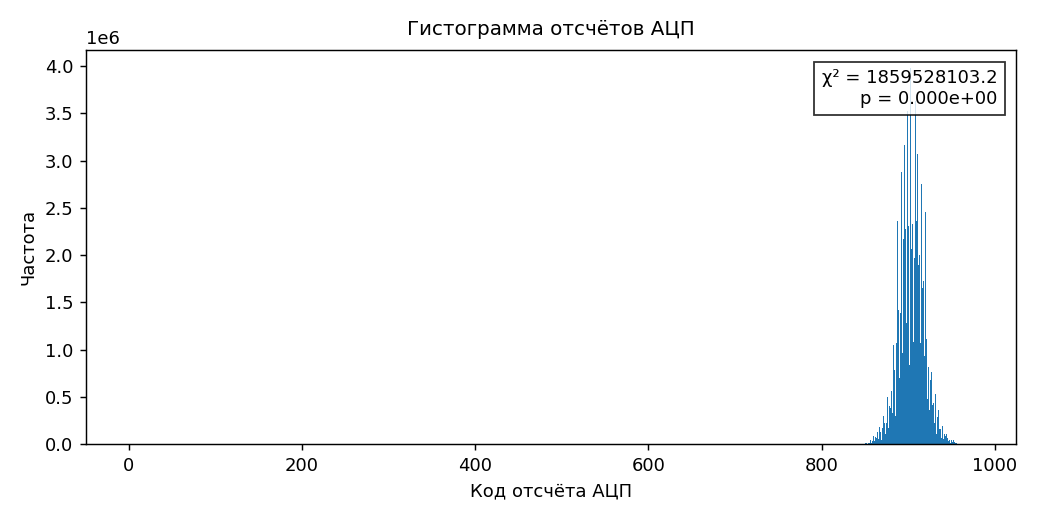
\includegraphics[width=\linewidth,keepaspectratio]{pandoc_media/media/exp_thermal_new/histogram_raw.png}
  \end{minipage}\hfill
  \begin{minipage}[t]{0.48\linewidth}
    \centering
    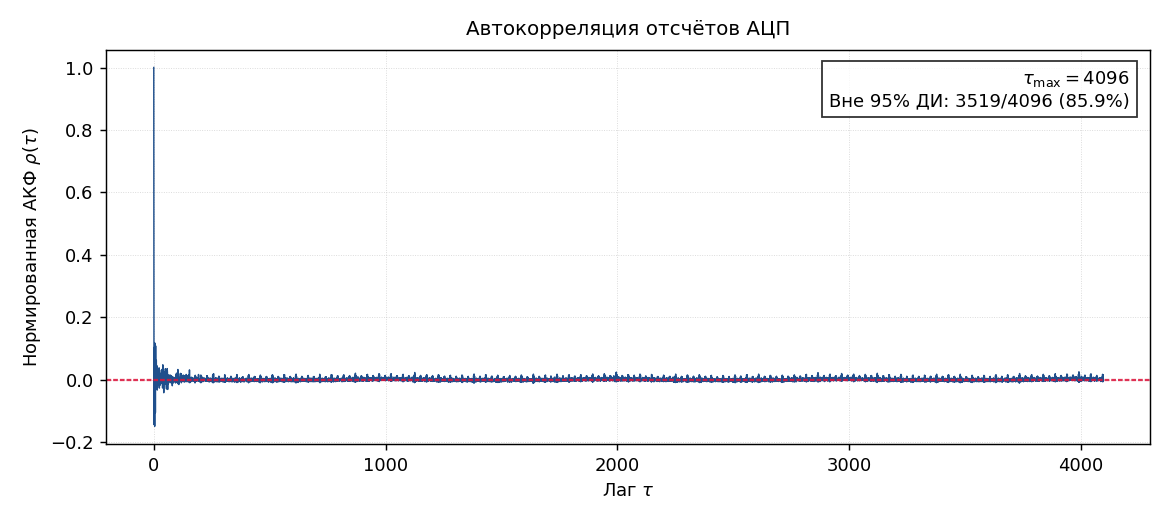
\includegraphics[width=\linewidth,keepaspectratio]{pandoc_media/media/exp_thermal_new/autocorr_raw.png}
  \end{minipage}
  \caption{Тепловой канал: гистограмма отсчётов АЦП
  ($N=85\cdot 10^6$) и нормированная автокорреляция отсчётов}
  \label{fig:thermal_new_hist}
\end{figure}

\begin{figure}[H]
  \centering
  
\includegraphics[width=0.55\linewidth,keepaspectratio]{pandoc_media/media/exp_thermal_new/bits_image.png}
  \caption{Визуализация фрагмента битового потока после извлечения МЗР и постобработки
  по схеме фон Неймана для теплового канала ($512\times512$~бит)}
  \label{fig:thermal_new_bitsmap}
\end{figure}

Распределение отсчётов узкое (стандартное отклонение менее $15$ единиц шкалы при
размахе $0\ldots 1023$) и заметно смещено к верхней границе диапазона: выборочное
среднее ${\approx}904$ из $1023$, что соответствует напряжению на входе АЦП
${\approx}4{,}4$~В. Природа обоих наблюдений напрямую связана с выбором
операционного усилителя.

\textbf{Смещение к 5~В.} TL072 при однополярном питании от $+12$~В не способен
вытянуть выход к нижнему рельсу: его минимальное выходное напряжение
ограничено величиной порядка $+1{,}5\ldots 2$~В (см.~раздел~3.3.5), что после
прохождения резистивной связи и второго каскада переводится в смещённую вверх
постоянную составляющую на входе АЦП. Иными словами, рабочая точка выхода
лежит \emph{не} вблизи геометрической середины шкалы ($V_\mathrm{mid}\approx
2{,}5$~В), а сдвинута почти на $2$~В вверх к границе диапазона АЦП. Этот
эффект --- неизбежная плата за выбор более <<тихого>> ОУ, и в данном опыте
не компенсировался смещением $V_\mathrm{mid}$ вниз (как это сделано для канала
BJT в разделе~3.5.4), поскольку для теплового канала важнее сохранить
естественное отношение сигнал/шум, чем выровнять гистограмму.

\textbf{Малая амплитуда.} Стандартное отклонение всего ${\approx}15$ единиц
АЦП (${\approx}73$~мВ на входе) при $G_\Sigma\approx 528$ означает, что
действующее напряжение шума на входе усилителя составляет лишь
${\approx}140$~мкВ --- крайне малая величина, того же порядка, что и
расчётный тепловой шум $10$~МОм-резистора (${\approx}64$~мкВ в полосе $24{,}8$~кГц)
плюс собственный шум входного каскада TL072 при работе с большим источниковым
сопротивлением. В этом и состоит главное практическое
ограничение теплового канала на резисторе: \emph{достигнутая в данной
постановке амплитуда близка к максимуму}, доступному без принципиальной
модификации схемы. Дальнейшие попытки увеличить $G$ заменой номиналов
обратной связи в наших экспериментах приводили к одному из двух исходов:
либо полное исчезновение полезного шума с выхода (тракт <<упирается>> в
ограничения по полосе и в собственный шум второго каскада), либо потеря
устойчивости тракта --- самовозбуждение на частоте полюса ОУ или дрейф
рабочей точки за пределы линейного диапазона. Поэтому для теплового канала
выбранная конфигурация рассматривается как практически предельная.

Автокорреляционная функция отсчётов содержит несколько узких <<резонансов>>
при малых задержках, ожидаемых при ограничении полосы и фильтрации шумов
цепями обратной связи, но в целом близка к шумовому профилю без устойчивых
периодических компонент.

\crssubhead{3.4.3. Сводка NIST STS}

Битовая последовательность была получена извлечением младшего разряда каждого
отсчёта и постобработкой по схеме фон Неймана. Результаты пакета NIST STS
($10\times 10^6$~бит) сведены в таблицу~\ref{tab:thermal_new_nist}.

\begin{table}[H]
  \centering
  \footnotesize
  \caption{NIST STS для теплового канала после фон Неймана. Сводка: PASS${}=10$,
  FAIL${}=5$, N/A${}=0$ (тесты RandomExcursions и RandomExcursionsVariant
  тривиально получают FAIL из-за несоответствия профиля случайных блужданий ---
  типичная особенность сильно сжатого VN-выхода)}
  \label{tab:thermal_new_nist}
  \begin{tabular}{|p{0.34\linewidth}|r|r|r|c|}
    \hline
    Группа тестов & Под\-тестов & min / max $p$ & Пройдено / всего & Вердикт \\
    \hline
    Frequency & 1 & $0{,}7399$ & $8/10$ & FAIL \\
    \hline
    BlockFrequency & 1 & $0{,}1223$ & $10/10$ & PASS \\
    \hline
    CumulativeSums & 2 & $0{,}5341$ -- $0{,}7399$ & $19/20$ & PASS \\
    \hline
    Runs & 1 & $0{,}0000$ & $0/10$ & FAIL \\
    \hline
    LongestRun & 1 & $0{,}0179$ & $10/10$ & PASS \\
    \hline
    Rank & 1 & $0{,}0179$ & $10/10$ & PASS \\
    \hline
    FFT & 1 & $0{,}2133$ & $10/10$ & PASS \\
    \hline
    NonOverlappingTemplate & 148 & $0{,}0000$ -- $0{,}9915$ & $1453/1480$ & FAIL \\
    \hline
    OverlappingTemplate & 1 & $0{,}1223$ & $10/10$ & PASS \\
    \hline
    Universal & 1 & $0{,}0669$ & $10/10$ & PASS \\
    \hline
    ApproximateEntropy & 1 & $0{,}2133$ & $10/10$ & PASS \\
    \hline
    RandomExcursions & 8 & --- & $40/40$ & FAIL \\
    \hline
    RandomExcursionsVariant & 18 & --- & $90/90$ & FAIL \\
    \hline
    Serial & 2 & $0{,}3505$ -- $0{,}5341$ & $20/20$ & PASS \\
    \hline
    LinearComplexity & 1 & $0{,}7399$ & $10/10$ & PASS \\
    \hline
  \end{tabular}
\end{table}

Несмотря на узость гистограммы, после фон Неймана из десяти содержательных групп
тестов (без учёта RandomExcursions, которые в данной постановке формально проваливаются
по техническим причинам --- см. пояснение к таблице) проходят восемь. Провал
\texttt{Runs} объясняется остаточной памятью процесса на коротких масштабах,
наследуемой от ограниченной полосы усилителя; провал \texttt{NonOverlapping\-Template}
характерен для тонкого смещения вероятностей появления отдельных коротких шаблонов
и в большинстве источников этой работы устранён только криптографическим
отбеливанием. Тем не менее тепловой канал в честной постановке демонстрирует
работоспособную энтропийную базу и хорошие оценки минимальной энтропии на бит
($0{,}9984$), достаточные для использования в качестве вспомогательного источника
при смешении с более <<живыми>> каналами.

\crssubhead{3.5. Лавинный шум обратносмещённого BE-перехода биполярного транзистора}

Лавинный пробой BE-перехода NPN-транзистора при обратном включении --- один из
наиболее изученных источников шума в любительских и коммерческих TRNG. В нём сочетаются
сразу несколько желательных свойств: высокая амплитуда импульсов (что упрощает
требования к усилителю и АЦП), широкополосный спектр, нечувствительность к
температурным колебаниям окружающей среды на масштабах сеанса записи и крайне низкая
стоимость элементной базы --- одного маломощного NPN-транзистора достаточно для всех
экспериментов раздела.

Именно этот источник стал основным предметом натурных исследований в работе, и ниже
последовательно прослеживается развитие конструкции усилительного тракта в четырёх
итерациях, причём каждая следующая итерация фиксирует и устраняет конкретный
артефакт, обнаруженный по результатам предыдущей. В качестве полупроводникового
прибора во всех экспериментах использовался NPN-транзистор BC337, включённый в
\emph{инвертированном} режиме с обратно смещённым BE-переходом: эмиттер через
балластный резистор $R_b=100$~кОм подтянут к шине $+12$~В, а коллектор и база
соединены с общим проводом (рисунок~\ref{fig:bjt_source_schema}). Лавинный
пробой развивается на BE-переходе при $U_{EB}\approx U_{CC}=12$~В; коллектор
посажен на землю для развязки и предотвращения накопления заряда на свободном
выводе, а ток пробоя ограничен балластным резистором $R_b$ со стороны эмиттера.
Полезный сигнал снимается с эмиттера через разделительный конденсатор
$C_1=0{,}1$~мкФ, который отрезает постоянную составляющую (${\approx}U_{BR}$ на
эмиттере) и передаёт на вход усилителя только переменную составляющую ---
случайные импульсы лавинных пробоев.

\textbf{Выбор экземпляра.} На начальном этапе предполагалось использовать
популярный 2N3904, у которого по справочным данным напряжение обратного пробоя
BE-перехода составляет $\sim 6\ldots 9$~В. Однако ни один из имевшихся под рукой
экземпляров 2N3904 не вышел в лавинный режим при штатном для стенда напряжении
питания $+12$~В: сигнал на выходе усилителя оставался на уровне собственного шума
тракта без характерных импульсов лавинного пробоя. После переключения на BC337
картина изменилась радикально --- лавинный режим устойчиво наблюдался при том же
$+12$~В без каких-либо дополнительных доработок схемы. Этот опыт хорошо
иллюстрирует тот факт, что заявленный в datasheet диапазон $U_{BR}$ относится к
параметрам кристалла в самом неблагоприятном случае, а фактическое напряжение
пробоя у конкретного экземпляра может оказаться существенно выше типового и
зависеть от партии. Для воспроизведения результатов раздела рекомендуется
именно BC337 (или ручной отбор экземпляров другой серии по факту попадания в
лавинный режим).

\crssubhead{3.5.1. Физическая модель и принципиальная схема}

При обратном смещении перехода $U_{BE,\,\text{rev}}$ выше напряжения пробоя
$U_{BR}$ (для BC337 при $U_{CC}=+12$~В лавинный режим устойчиво достижим) начинается ударная
ионизация: ускоренный электрическим полем электрон выбивает из кристаллической
решётки новую пару электрон--дырка, и процесс <<размножается>>. Поскольку число
новых носителей в каждой лавине случайно, через переход течёт случайно
флуктуирующий ток в диапазоне ${\sim}10\ldots 50$~мкА (грубая оценка
$(U_{CC}-U_{BR})/R_b$ при $U_{CC}=12$~В и $U_{BR}\!\sim\!7\ldots 9$~В для
BC337) со спектральной плотностью дробового типа с увеличением множителем
избыточного шума $F$ (см.~формулу $S_I(f)=2qIM^2F$, раздел~2.1). На балластном
сопротивлении $R_b=100$~кОм этот ток создаёт случайное напряжение, которое
усиливается операционными каскадами и оцифровывается АЦП.

\begin{figure}[H]
  \centering
  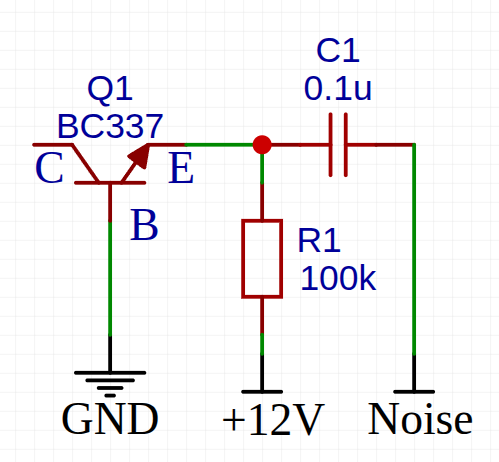
\includegraphics[width=0.55\linewidth,keepaspectratio]{pandoc_media/media/bjt_noise_source/schema.png}
  \caption{Принципиальная схема источника лавинного шума BJT. Транзистор
  Q1 = BC337 включён инвертированно: коллектор C и база B соединены с GND,
  эмиттер E через балластный резистор $R_1\equiv R_b=100$~кОм подключён к
  шине $+12$~В. Полезный сигнал снимается с эмиттера через разделительный
  конденсатор $C_1=0{,}1$~мкФ и подаётся на вход усилителя (точка <<Noise>>
  схемы рисунка~\ref{fig:amp_2stage})}
  \label{fig:bjt_source_schema}
\end{figure}

Источник шума оформлен как самостоятельный модуль, выход которого
(<<Noise>>) соединяется со входом усилительного тракта раздела~3.3
(точка <<Noise>> на схеме рисунка~\ref{fig:amp_2stage}). Питание $+12$~В
одновременно обеспечивает обратное смещение BE-перехода (для пробоя) и
питание операционных каскадов усилителя; общая земля стенда объединяет
землю $+12$~В, землю Arduino и общий провод усилителя.

\crssubhead{3.5.2. Этап 1 --- одиночный каскад усиления}

В первой итерации использовался однокаскадный неинвертирующий усилитель на LM358
с $R_g=10$~кОм, $R_f=470$~кОм (см.~рисунок~\ref{fig:amp_1stage} раздела~3.3.2),
что даёт коэффициент усиления $G=1+R_f/R_g\approx 48$. Гипотеза: даже относительно
скромного усиления окажется достаточно, чтобы лавинные импульсы стали различимы
младшими разрядами АЦП. Результаты сеанса сведены в
таблице~\ref{tab:bjt_stage1_summary}.

\begin{table}[H]
  \centering
  \footnotesize
  \caption{Этап 1: однокаскадный усилитель ($G\approx 48$), LM358}
  \label{tab:bjt_stage1_summary}
  \begin{tabular}{|p{0.55\linewidth}|p{0.35\linewidth}|}
    \hline
    Число отсчётов & $85\cdot 10^6$ \\
    \hline
    Среднее по шкале АЦП & $476{,}2$ \\
    \hline
    Стандартное отклонение $\sigma_\mathrm{adc}$ & $28{,}3$ \\
    \hline
    Минимум / максимум по выборке & $256$ / $767$ \\
    \hline
    Медиана PSD ($f_s\approx 49{,}6$~кГц) & $3{,}4\cdot 10^{-2}$ \\
    \hline
    Шеннон / минимальная энтропия на бит (VN) & $1{,}0000$ / $0{,}9994$ \\
    \hline
  \end{tabular}
\end{table}

\begin{figure}[H]
  \centering
  \begin{minipage}[t]{0.48\linewidth}
    \centering
    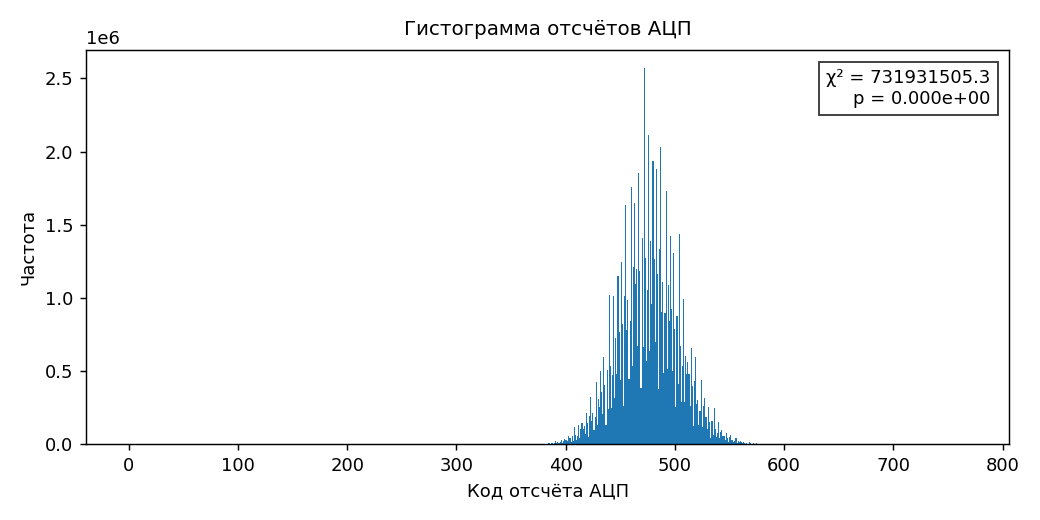
\includegraphics[width=\linewidth,keepaspectratio]{pandoc_media/media/exp_bjt_1stage/histogram_raw.png}
  \end{minipage}\hfill
  \begin{minipage}[t]{0.48\linewidth}
    \centering
    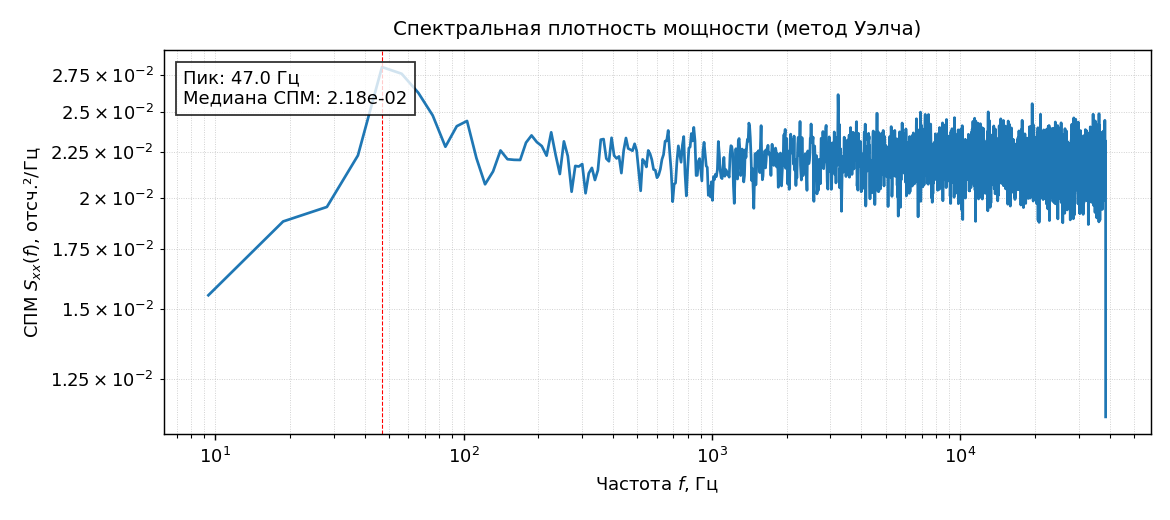
\includegraphics[width=\linewidth,keepaspectratio]{pandoc_media/media/exp_bjt_1stage/psd_raw.png}
  \end{minipage}
  \caption{Этап 1 (одиночный каскад): гистограмма отсчётов АЦП и оценка
  спектральной плотности мощности}
  \label{fig:bjt_stage1_plots}
\end{figure}

Основная масса полезного сигнала сосредоточена в окрестности середины шкалы
АЦП и укладывается в окно ${\sim}\pm 3\sigma_\mathrm{adc}\approx\pm 85$ единиц
вокруг среднего, что соответствует ${\sim}20\%$ полного $10$-битного диапазона
(редкие выбросы во всём наборе из $85\cdot 10^6$ отсчётов достигают границ $256$
и $767$). При коэффициенте усиления $G\approx 48$ это означает, что
действующее напряжение шума на входе усилителя составляет
$\sigma_\mathrm{adc}\cdot(5\text{ В}/1024)/G\approx 3$~мВ, а характерный размах
лавинных импульсов на входе --- порядка $20$~мВ при полной шкале АЦП $5$~В на
выходе. По результатам NIST STS поток МЗР без постобработки даёт ожидаемо плохой
профиль (PASS${}=2$, FAIL${}=11$, N/A${}=2$), однако после фон Неймана
восстанавливается до приемлемого уровня (PASS${}=12$, FAIL${}=3$, N/A${}=0$):
провалы остаются только в NonOverlapping\-Template и RandomExcursions
(последний по техническим причинам теста). Вывод этапа --- источник
работоспособен по сути, но коэффициент усиления $G\approx 48$ субоптимален:
большая часть шкалы АЦП простаивает, что увеличивает вклад статической квантовой
ошибки относительно полезного сигнала.

\crssubhead{3.5.3. Этап 2 --- переход на двухкаскадный усилитель}

Следующий шаг --- добавление второго неинвертирующего каскада на втором канале
того же LM358 с $R_{g2}=R_4=10$~кОм, $R_{f2}=R_6=100$~кОм; собственное усиление
второго каскада $G_2=1+R_{f2}/R_{g2}\approx 11$. Выход первого каскада подаётся
на инвертирующий вход второго через последовательный резистор $R_4=10$~кОм
(резистивная связь без AC-разделения, см.~раздел~3.3.3 и рисунок~\ref{fig:amp_2stage}).
Суммарное усиление возросло до $G_\Sigma\approx 48\cdot 11\approx 528$.
Результаты сеанса приведены в таблице~\ref{tab:bjt_stage2_summary} и на
рисунке~\ref{fig:bjt_stage2_plots}.

\begin{table}[H]
  \centering
  \footnotesize
  \caption{Этап 2: двухкаскадный усилитель ($G_\Sigma\approx 528$), LM358}
  \label{tab:bjt_stage2_summary}
  \begin{tabular}{|p{0.55\linewidth}|p{0.35\linewidth}|}
    \hline
    Число отсчётов & $85\cdot 10^6$ \\
    \hline
    Среднее по шкале АЦП & $596{,}4$ \\
    \hline
    Стандартное отклонение $\sigma_\mathrm{adc}$ & $145{,}3$ \\
    \hline
    Минимум / максимум по выборке & $0$ / $1023$ (наблюдается насыщение) \\
    \hline
    Шеннон / минимальная энтропия на бит (VN) & $1{,}0000$ / $0{,}9998$ \\
    \hline
    NIST STS (VN): PASS / FAIL / N/A & $13$ / $2$ / $0$ \\
    \hline
  \end{tabular}
\end{table}

\begin{figure}[H]
  \centering
  \begin{minipage}[t]{0.48\linewidth}
    \centering
    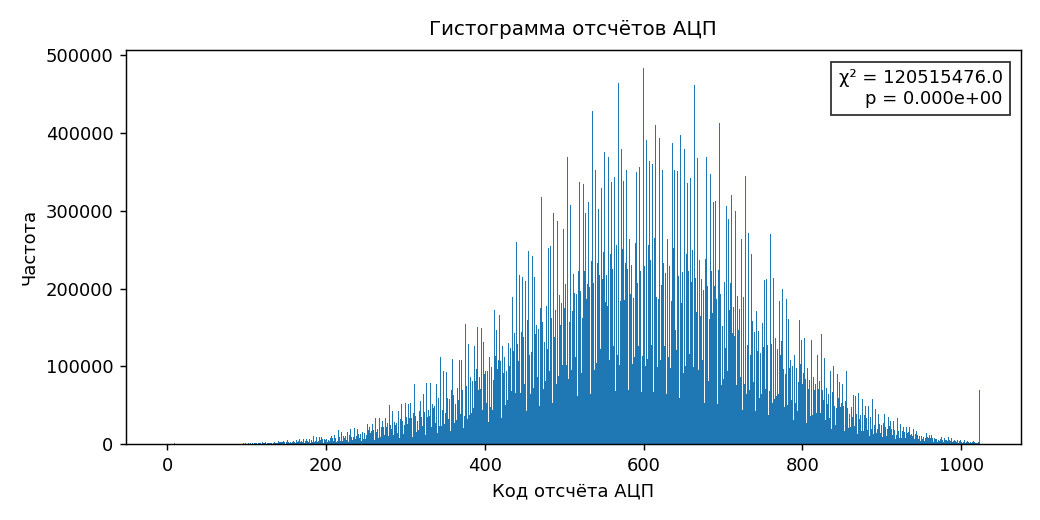
\includegraphics[width=\linewidth,keepaspectratio]{pandoc_media/media/exp_bjt_2stage/histogram_raw.png}
  \end{minipage}\hfill
  \begin{minipage}[t]{0.48\linewidth}
    \centering
    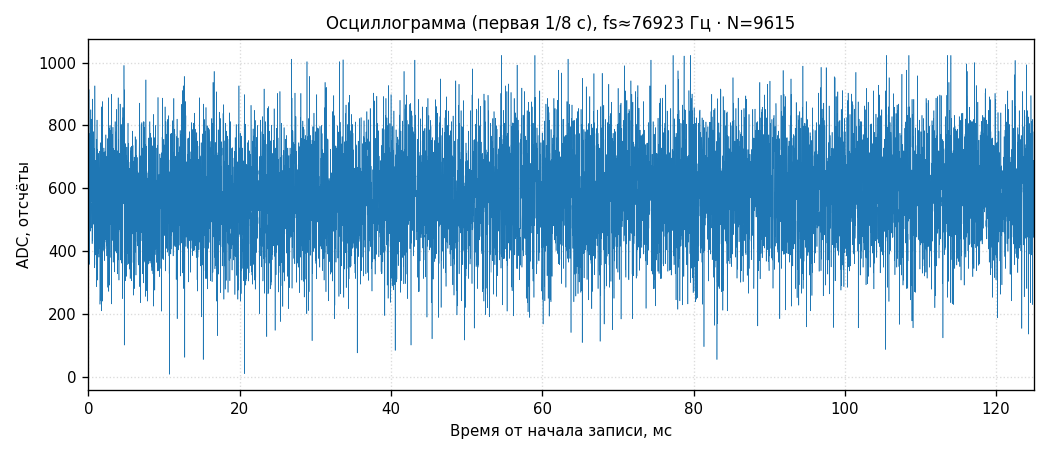
\includegraphics[width=\linewidth,keepaspectratio]{pandoc_media/media/exp_bjt_2stage/scope_time_125ms.png}
  \end{minipage}
  \caption{Этап 2 (двухкаскадный усилитель): гистограмма отсчётов АЦП и
  осциллограмма первых $125$~мс записи. На гистограмме видна выраженная аномалия ---
  накопление отсчётов на верхней границе шкалы (значение $1023$); на осциллограмме
  заметно <<упирание>> сигнала в потолок}
  \label{fig:bjt_stage2_plots}
\end{figure}

Качественно профиль изменился радикально: стандартное отклонение возросло в пять раз
(с $28$ до $145$), диапазон значений теперь занимает практически всю шкалу АЦП, а
NIST STS показывает $13$ PASS / $2$ FAIL / $0$ N/A --- лучший результат среди всех
постановок этого канала на данный момент. Однако на гистограмме отчётливо проявляется
\emph{нежелательная} особенность: высокий и узкий пик на правой границе диапазона
(значение $1023$). Это \emph{не} физический эффект источника, а артефакт усилителя:
выход второго каскада LM358 при питании $+5$~В физически не может подниматься выше
${\approx}3{,}5$~В (раздел~3.3.5), и одновременно <<обычная>> постоянная составляющая
тракта, унаследованная от $V_\mathrm{mid}\approx 2{,}5$~В, оставляет на верхней
половине шкалы недостаточный запас. В результате положительные полуволны лавинных
импульсов начинают систематически срезаться, и АЦП регистрирует их как насыщенное
значение $1023$.

Этот класс артефакта особенно неприятен для последующей постобработки: насыщение ---
\emph{детерминированный} процесс, и младшие биты насыщенных отсчётов несут не
случайную информацию (их значение жёстко равно $1$ при выходе на верхний предел и
$1$ для значения $1023$). Поэтому несмотря на формально лучший результат NIST STS,
такая конфигурация требует исправления.

\crssubhead{3.5.4. Этап 3 --- коррекция $V_\mathrm{mid}$ для устранения насыщения}

Логика следующей итерации проста: чтобы доступное окно линейности выхода LM358 стало
\emph{симметричным} относительно текущего среднего, нужно сместить $V_\mathrm{mid}$
вниз --- так, чтобы расстояние от $V_\mathrm{mid}$ до фактического верхнего рельса
LM358 (${\approx}3{,}5$~В) стало равно расстоянию от $V_\mathrm{mid}$ до нуля.
Аналитически оптимум при $U_\mathrm{out,\,max}=3{,}5$~В лежит вблизи
$V_\mathrm{mid}\approx 1{,}75$~В.

Поскольку к моменту обнаружения артефакта насыщения на этапе~2 макетная плата
стенда уже была полностью смонтирована и испытана, было принято решение реализовать
требуемое смещение \emph{без перепайки} исходного делителя. К нижнему резистору
делителя $R_2=10$~кОм был добавлен ещё один резистор $10$~кОм, включённый
параллельно: точка $V_\mathrm{mid}$ оказалась подтянута к земле через эквивалентное
сопротивление $R_2\,\|\,10\text{ кОм} = 5$~кОм, и опорное напряжение делителя
составило
\begin{equation}
  V_\mathrm{mid}
  = U_{CC}\cdot\dfrac{R_2\,\|\,10\text{ кОм}}{R_1+R_2\,\|\,10\text{ кОм}}
  = 5\text{ В}\cdot\dfrac{5\text{ кОм}}{10\text{ кОм}+5\text{ кОм}}
  \approx 1{,}67\text{ В}.
\end{equation}
Такая модификация вносит минимальное вмешательство в уже отлаженный макет ---
один навесной резистор поверх существующего --- и одновременно даёт оптимальное
по симметрии гистограммы смещение рабочей точки. Аналогичного результата можно
достичь штатной заменой $R_2$ на $5{,}1$~кОм; вариант с добавлением параллельного
резистора был выбран как более быстрый в условиях итеративной отладки.

Результаты сеанса после внесения этой коррекции приведены в
таблице~\ref{tab:bjt_stage3_summary} и на рисунке~\ref{fig:bjt_stage3_plots}.

\begin{table}[H]
  \centering
  \footnotesize
  \caption{Этап 3: двухкаскадный усилитель ($G_\Sigma\approx 528$), LM358,
  $V_\mathrm{mid}\approx 1{,}67$~В}
  \label{tab:bjt_stage3_summary}
  \begin{tabular}{|p{0.55\linewidth}|p{0.35\linewidth}|}
    \hline
    Число отсчётов & $85\cdot 10^6$ \\
    \hline
    Среднее по шкале АЦП & $516{,}3$ \\
    \hline
    Стандартное отклонение $\sigma_\mathrm{adc}$ & $122{,}1$ \\
    \hline
    Минимум / максимум по выборке & $0$ / $1023$ (насыщение ослаблено) \\
    \hline
    Шеннон / минимальная энтропия на бит (VN) & $1{,}0000$ / $0{,}9999$ \\
    \hline
    NIST STS (VN): PASS / FAIL / N/A & $12$ / $3$ / $0$ \\
    \hline
  \end{tabular}
\end{table}

\begin{figure}[H]
  \centering
  \begin{minipage}[t]{0.48\linewidth}
    \centering
    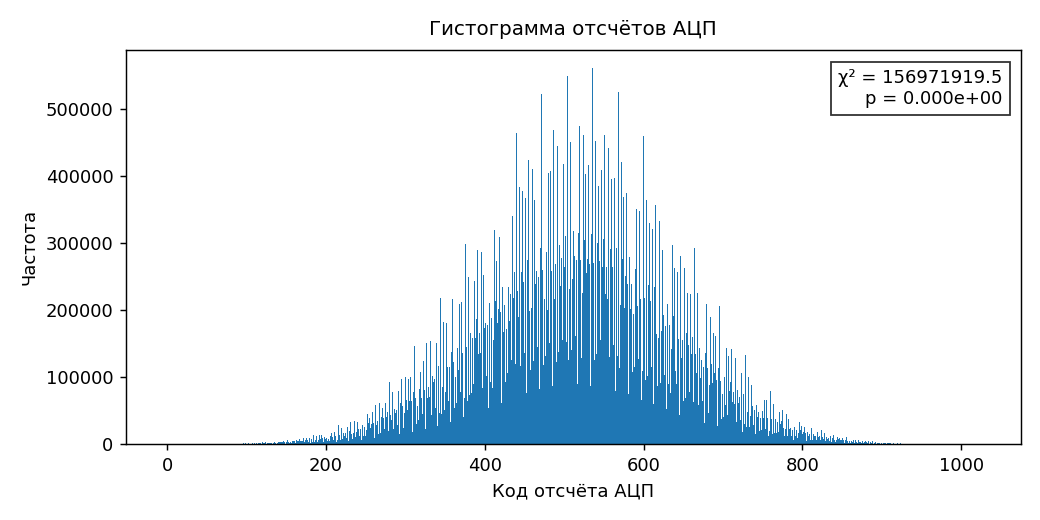
\includegraphics[width=\linewidth,keepaspectratio]{pandoc_media/media/exp_bjt_bias_tune/histogram_raw.png}
  \end{minipage}\hfill
  \begin{minipage}[t]{0.48\linewidth}
    \centering
    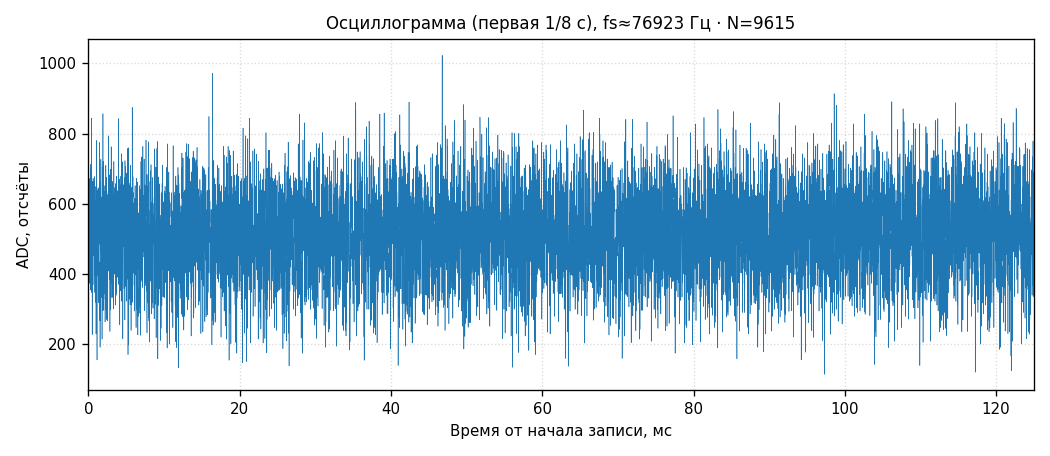
\includegraphics[width=\linewidth,keepaspectratio]{pandoc_media/media/exp_bjt_bias_tune/scope_time_125ms.png}
  \end{minipage}
  \caption{Этап 3 (коррекция $V_\mathrm{mid}$): гистограмма стала практически
  симметричной, на осциллограмме <<упирания>> в потолок более не наблюдается}
  \label{fig:bjt_stage3_plots}
\end{figure}

Гистограмма приобрела квазигауссовский вид с симметричными хвостами; пик у границы
$1023$ практически исчез. Стандартное отклонение немного уменьшилось ($145\to 122$) ---
ожидаемо, поскольку статистический вклад в дисперсию вносили насыщенные отсчёты
(их теперь нет). NIST STS дал $12$ PASS / $3$ FAIL / $0$ N/A --- формально
немного хуже, чем на этапе 2, однако \emph{результаты этапа 3 уже отражают чистый
вклад физического источника}, а не комбинацию шума и систематического отсечения.

\crssubhead{3.5.5. Этап 4 --- стабилизация питания и финальная конфигурация}

В четвёртой итерации усилительный тракт стенда был сохранён без изменений, но
дополнительно введена тщательная развязка по питанию: на шине $+5$~В перед усилителем
поставлен LC-фильтр (дроссель $10$~мкГн $+$ ферритовая бусина $+$ электролит
$100$~мкФ $+$ керамика $0{,}1$~мкФ), а на шине $+12$~В (источник для пробоя BJT)
установлен RC-фильтр и танталовый конденсатор $22$~мкФ. Цель --- устранить
просачивание импульсных помех от USB-питания платы в усилительный тракт и
дополнительно стабилизировать рабочую точку пробоя транзистора. Эта
конфигурация принята как \emph{итоговая} для канала; именно её данные
используются в качестве референса для всех дальнейших экспериментов и для
сравнительной таблицы раздела~3.9.

\begin{table}[H]
  \centering
  \footnotesize
  \caption{Этап 4: финальная конфигурация ($G_\Sigma\approx 528$), LM358,
  $V_\mathrm{mid}\approx 1{,}67$~В, развязка по питанию}
  \label{tab:bjt_stage4_summary}
  \begin{tabular}{|p{0.55\linewidth}|p{0.35\linewidth}|}
    \hline
    Число отсчётов & $85\cdot 10^6$ \\
    \hline
    Среднее по шкале АЦП & $505{,}4$ \\
    \hline
    Стандартное отклонение $\sigma_\mathrm{adc}$ & $146{,}5$ \\
    \hline
    Минимум / максимум по выборке & $0$ / $1023$ (физический разброс) \\
    \hline
    Медиана PSD ($f_s\approx 49{,}6$~кГц) & $8{,}5\cdot 10^{-1}$ \\
    \hline
    Шеннон / минимальная энтропия на бит (VN) & $1{,}0000$ / $0{,}9999$ \\
    \hline
    Шеннон / минимальная энтропия на байт (VN) & $7{,}9999$ / $7{,}9571$ \\
    \hline
    NIST STS (VN): PASS / FAIL / N/A & $\mathbf{13}$ / $\mathbf{2}$ / $\mathbf{0}$ \\
    \hline
  \end{tabular}
\end{table}

\begin{figure}[H]
  \centering
  \begin{minipage}[t]{0.48\linewidth}
    \centering
    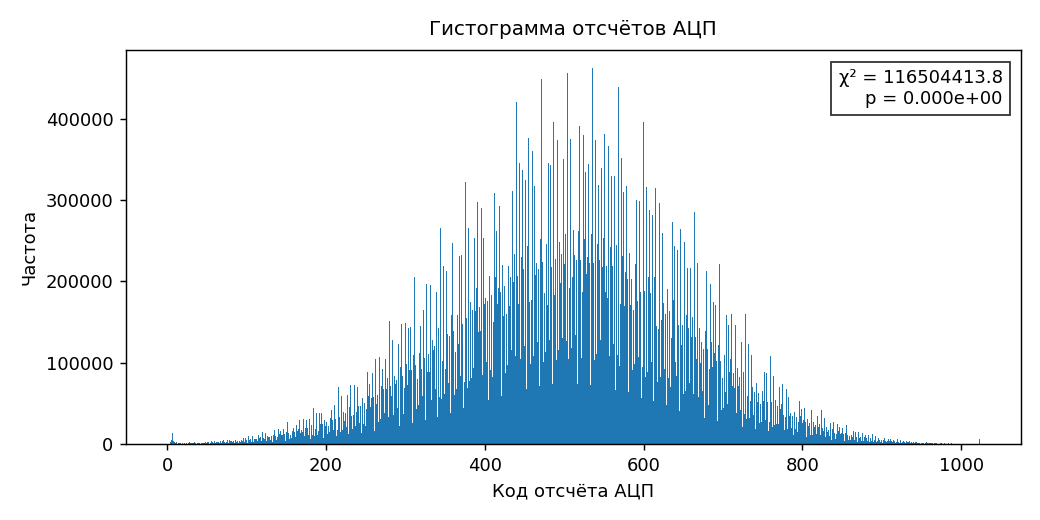
\includegraphics[width=\linewidth,keepaspectratio]{pandoc_media/media/exp_bjt_vcc_stab/histogram_raw.png}
  \end{minipage}\hfill
  \begin{minipage}[t]{0.48\linewidth}
    \centering
    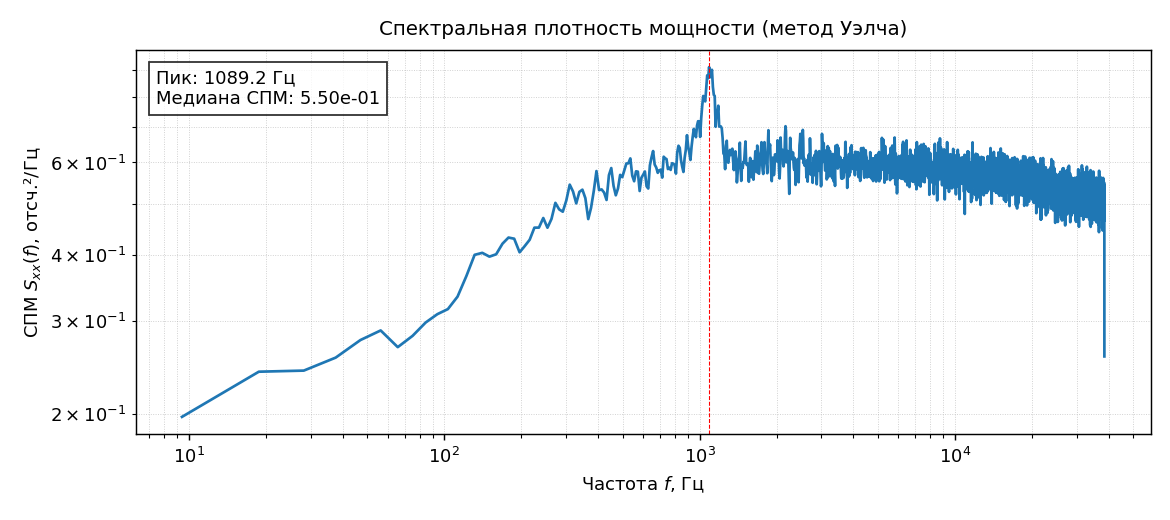
\includegraphics[width=\linewidth,keepaspectratio]{pandoc_media/media/exp_bjt_vcc_stab/psd_raw.png}
  \end{minipage}
  \caption{Финальная конфигурация (этап 4): гистограмма и оценка спектральной
  плотности мощности. Распределение симметрично, спектр близок к плоскому в
  рабочей полосе}
  \label{fig:bjt_stage4_plots}
\end{figure}

\begin{figure}[H]
  \centering
  
\includegraphics[width=0.55\linewidth,keepaspectratio]{pandoc_media/media/exp_bjt_vcc_stab/bits_image.png}
  \caption{Визуализация фрагмента битового потока после извлечения МЗР и
  постобработки по схеме фон Неймана для итоговой конфигурации канала BJT
  ($512\times512$ бит). Визуально структура неотличима от равномерного <<белого>>
  шума}
  \label{fig:bjt_stage4_bitsmap}
\end{figure}

Развёрнутая сводка NIST STS для итоговой конфигурации приведена в
таблице~\ref{tab:bjt_stage4_nist}.

\begin{table}[H]
  \centering
  \footnotesize
  \caption{NIST STS для финальной конфигурации канала BJT после фон Неймана.
  Сводка: PASS${}=13$, FAIL${}=2$, N/A${}=0$. Провалы RandomExcursions и
  RandomExcursionsVariant имеют технический характер (см.~раздел~3.4.3)}
  \label{tab:bjt_stage4_nist}
  \begin{tabular}{|p{0.34\linewidth}|r|r|r|c|}
    \hline
    Группа тестов & Под\-тестов & min / max $p$ & Пройдено / всего & Вердикт \\
    \hline
    Frequency & 1 & $0{,}2133$ & $10/10$ & PASS \\
    \hline
    BlockFrequency & 1 & $0{,}7399$ & $10/10$ & PASS \\
    \hline
    CumulativeSums & 2 & $0{,}2133$ -- $0{,}7399$ & $20/20$ & PASS \\
    \hline
    Runs & 1 & $0{,}2133$ & $10/10$ & PASS \\
    \hline
    LongestRun & 1 & $0{,}7399$ & $10/10$ & PASS \\
    \hline
    Rank & 1 & $0{,}0669$ & $9/10$ & PASS \\
    \hline
    FFT & 1 & $0{,}5341$ & $10/10$ & PASS \\
    \hline
    NonOverlappingTemplate & 148 & $0{,}0002$ -- $0{,}9915$ & $1466/1480$ & PASS \\
    \hline
    OverlappingTemplate & 1 & $0{,}5341$ & $10/10$ & PASS \\
    \hline
    Universal & 1 & $0{,}1223$ & $10/10$ & PASS \\
    \hline
    ApproximateEntropy & 1 & $0{,}5341$ & $10/10$ & PASS \\
    \hline
    RandomExcursions & 8 & --- & $48/48$ & FAIL \\
    \hline
    RandomExcursionsVariant & 18 & --- & $108/108$ & FAIL \\
    \hline
    Serial & 2 & $0{,}1223$ -- $0{,}9114$ & $20/20$ & PASS \\
    \hline
    LinearComplexity & 1 & $0{,}5341$ & $10/10$ & PASS \\
    \hline
  \end{tabular}
\end{table}

\crssubhead{3.5.6. Эволюция результатов и обсуждение}

Прогресс четырёх итераций сведён в таблице~\ref{tab:bjt_evolution}: видно, как каждая
итерация целенаправленно <<выбирала>> по одному наблюдаемому артефакту предыдущей
постановки.

\begin{table}[H]
  \centering
  \scriptsize
  \setlength{\tabcolsep}{3pt}
  \caption{Эволюция канала BJT по итерациям}
  \label{tab:bjt_evolution}
  \begin{tabular}{|p{0.04\linewidth}|p{0.20\linewidth}|p{0.08\linewidth}|p{0.10\linewidth}|p{0.07\linewidth}|p{0.26\linewidth}|}
    \hline
    Эт. & Конфигурация & $\sigma_\mathrm{adc}$ & NIST (VN) & Насы\-щение & Что сделано/выявлено \\
    \hline
    1 & 1 каскад, $G\!\approx\!48$ & $28{,}3$ & 12/3/0 & нет & низкая амплитуда: рабочее окно ${\sim}\pm 3\sigma\approx 20\%$ шкалы АЦП \\
    \hline
    2 & 2 каскада, $G\!\approx\!528$ & $145{,}3$ & 13/2/0 & \emph{да} ($1023$) & проявился потолок LM358; формальный STS улучшился, но за счёт детерминированных насыщенных отсчётов \\
    \hline
    3 & 2 каскада, $V_\mathrm{mid}\!\approx\!1{,}67$~В & $122{,}1$ & 12/3/0 & нет & симметричная гистограмма, чистый физический сигнал \\
    \hline
    4 & + развязка по питанию & $146{,}5$ & \textbf{13/2/0} & нет & итоговая конфигурация: лучший результат при честной форме распределения \\
    \hline
  \end{tabular}
\end{table}

Главный методический урок этой последовательности: формальные показатели NIST STS
не следует трактовать в отрыве от физической формы сигнала. На этапе 2 пакет STS
выдал лучший результат, чем на этапе 1, --- но именно благодаря неустранимому
систематическому артефакту (насыщению), который при последующем усложнении сценария
обработки (например, при отбеливании XOR с другим источником, при работе через
второй фон Нейман, при пересжатии криптографическим хэшем) проявил бы себя как
коррелированный смещающий вклад. Этап 3 \emph{ухудшил} формальные показатели на одну
группу, но сделал источник пригодным для дальнейшего использования, что и
подтверждается успешным этапом 4.

Финальная конфигурация была собрана навесным монтажом на универсальной перфорированной
макетной плате (\textit{perfboard}, шаг отверстий $2{,}54$~мм) с точечной пайкой и
проволочными перемычками; именно эта <<распайка>> использовалась для всех записей
этапа~4 и для прогона двухступенчатой постобработки раздела~3.5.8. Коррекция
$V_\mathrm{mid}$, описанная в разделе~3.5.4, выполнена непосредственно поверх
готовой платы --- добавочный резистор $10$~кОм припаян параллельно нижнему плечу
делителя без демонтажа исходного резистора.

\begin{figure}[H]
  \centering
  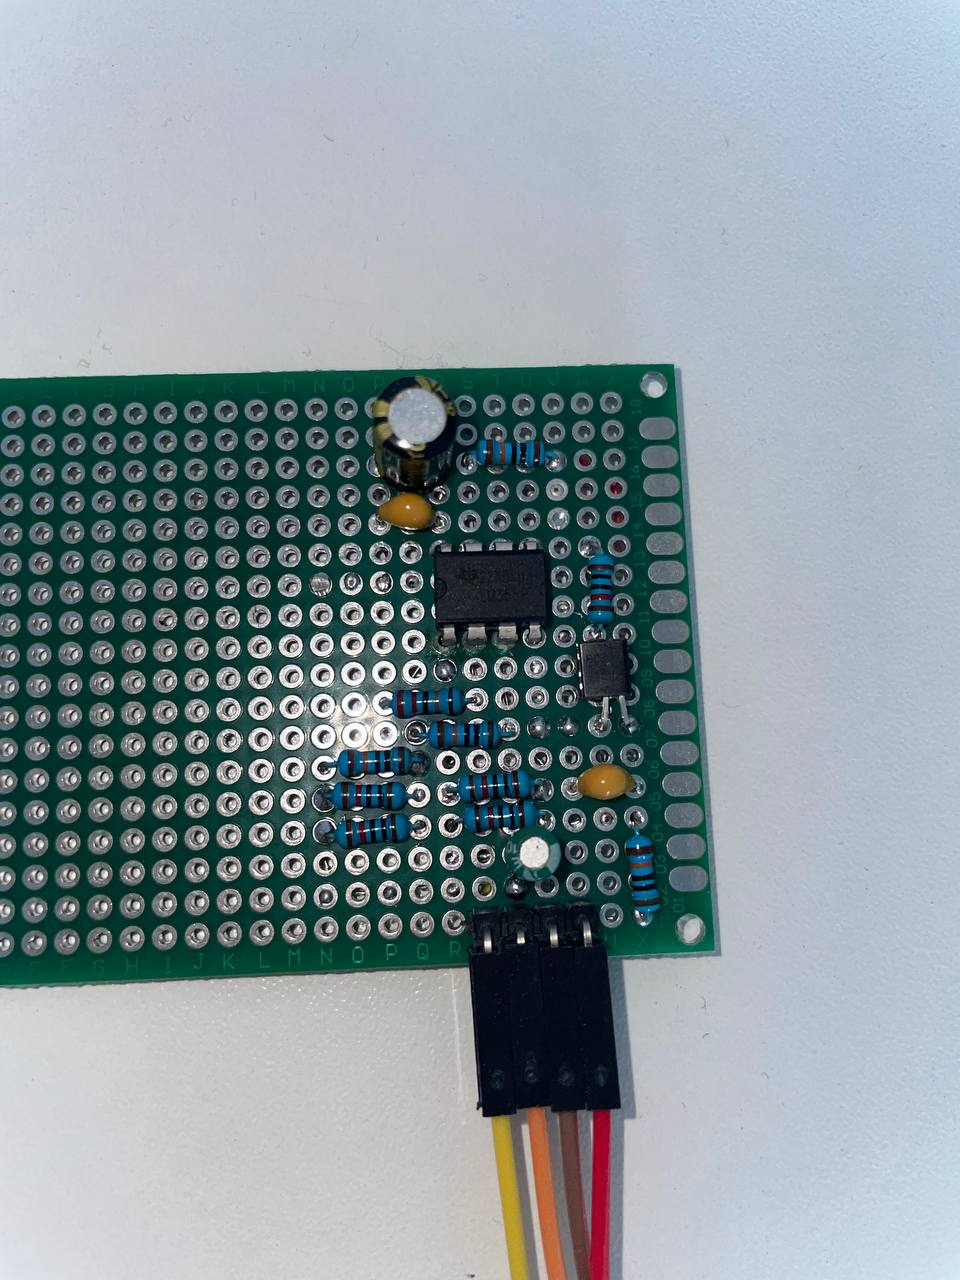
\includegraphics[width=0.55\linewidth,keepaspectratio]{pandoc_media/media/photo_trng_bjt_module/board.jpg}
  \caption{Фотография финальной распайки модуля канала BJT на универсальной
  перфорированной макетной плате. В кадре видны: микросхема операционного
  усилителя в DIP-8 корпусе (LM358, двухкаскадный неинвертирующий усилитель),
  транзистор Q1 = BC337 (TO-92), балластный резистор $R_b=100$~кОм
  источника шума, металлоплёночные резисторы цепей обратной связи и делителя
  $V_\mathrm{mid}$, развязывающие конденсаторы по питанию и 4-контактный
  штыревой разъём для подключения к Arduino Nano (питание $+12$~В, общий
  провод и сигнал на вход АЦП A0)}
  \label{fig:bjt_pcb_photo}
\end{figure}

\crssubhead{3.5.7. Однопроходная постобработка сырого потока МЗР}

В качестве альтернативы базовой схеме фон Неймана для итогового сеанса этапа~4 были
опробованы несколько способов прямого отбеливания потока МЗР --- каждый из методов
применялся напрямую к выходу процедуры извлечения младших разрядов, без
предварительной коррекции по фон Нейману. Сводные результаты по числу пройденных
групп тестов NIST STS приведены в таблице~\ref{tab:bjt_postproc_compare}.

\begin{table}[H]
  \centering
  \scriptsize
  \setlength{\tabcolsep}{3pt}
  \caption{Однопроходная постобработка сырого МЗР для итогового сеанса канала BJT
  (этап~4 раздела~3.5.5)}
  \label{tab:bjt_postproc_compare}
  \begin{tabular}{|p{0.28\linewidth}|p{0.42\linewidth}|c|c|c|}
    \hline
    Метод & Краткое описание & PASS & FAIL & N/A \\
    \hline
    von Neumann (базовый) & пары $(0,1)\!\to\! 0$, $(1,0)\!\to\! 1$, прочие отбрасываются & 13 & 2 & 0 \\
    \hline
    \texttt{decim\_xor8win} & XOR восьми последовательных МЗР $\to$ 1 бит выхода & 12 & 3 & 0 \\
    \hline
    \texttt{sha256\_2048} & SHA-256 от блоков сырых данных по $2048$~B & 12 & 3 & 0 \\
    \hline
    \texttt{xor\_delay8} & $b'_i = b_i \oplus b_{i-8}$ & 9 & 6 & 0 \\
    \hline
    \texttt{xor\_lsb012} & XOR трёх младших разрядов одного отсчёта & 8 & 5 & 2 \\
    \hline
    \texttt{fold\_lsb\_byte} & XOR-сложение в байты + xorshift отбеливание & 2 & 11 & 2 \\
    \hline
  \end{tabular}
\end{table}

Среди опробованных однопроходных методов лидером по количеству пройденных групп
тестов оказался фон Нейман, причём он не уступает ни криптографическому хэшу
SHA-256, ни XOR-децимации с окном 8. Однако ни один из перечисленных способов в
одиночку не позволяет добиться полного прохождения NIST STS: остаются провалы в
группах RandomExcursions и RandomExcursionsVariant, отражающие тонкую остаточную
структуру битового потока. Эти результаты подвели нас к следующему естественному
шагу --- каскадированию двух процедур постобработки.

\crssubhead{3.5.8. Двухступенчатая постобработка: фон Нейман + второй проход}

Логика следующего эксперимента такова. Постобработка по фон Нейману устраняет
самое грубое нарушение --- асимметрию вероятностей $p(0)\neq p(1)$ на уровне
отдельных битов, но не борется с локальной памятью процесса и тонкими структурными
артефактами, накладываемыми ограниченной полосой усилителя. Если за фон Нейманом
поставить ещё один проход децимирующего отбеливания (XOR или эквивалентного),
второй проход должен <<съесть>> уже именно остаточные корреляции, доступные после
первой коррекции. Каждый из четырёх алгоритмов раздела~3.5.7 был применён повторно
к выходу постобработки фон Неймана. Сводные результаты пакета NIST STS
приведены в таблице~\ref{tab:bjt_postproc_after_vn}.

\begin{table}[H]
  \centering
  \scriptsize
  \setlength{\tabcolsep}{3pt}
  \caption{Двухступенчатая постобработка (фон Нейман $+$ второй проход) для
  итогового сеанса канала BJT (этап~4 раздела~3.5.5). На входе второй
  ступени --- $\approx 4{,}25\cdot 10^7$ бит выхода фон Неймана; на каждый
  прогон NIST STS взяты стандартные $10\times 10^6$~бит}
  \label{tab:bjt_postproc_after_vn}
  \begin{tabular}{|p{0.26\linewidth}|p{0.40\linewidth}|c|c|c|}
    \hline
    Второй проход после VN & Краткое описание & PASS & FAIL & N/A \\
    \hline
    \texttt{xor\_delay8} & $b'_i = b_i\oplus b_{i-8}$ по выходу VN & 13 & 2 & 0 \\
    \hline
    \texttt{xor\_lsb012} & скользящий XOR трёх подряд бит выхода VN & 13 & 2 & 0 \\
    \hline
    \texttt{decim\_xor8win} & 1 бит выхода $=$ XOR из 8 подряд бит VN & \textbf{15} & \textbf{0} & \textbf{0} \\
    \hline
    \texttt{fold\_lsb\_byte} & побайтовое XOR-сложение $+$ xorshift отбеливание & \textbf{15} & \textbf{0} & \textbf{0} \\
    \hline
    \texttt{sha256\_2048} & SHA-256 блоков по $2048$~B файла после VN & --- & --- & --- \\
    \hline
  \end{tabular}
\end{table}

Прогон по методу \texttt{sha256\_2048} прервался на длине входа: после двойной
постобработки (VN дал $\approx 6{,}2$~МБ, а 1:64-я компрессия SHA сократила это до
${\approx}0{,}5$~МБ) выход оказался короче минимума $1{,}25$~МБ, требуемого для
полного STS при $10\times 10^6$ бит. Этот результат отдельно подчёркивает
практическую цену каскадной постобработки: каждое последующее звено агрессивно
сокращает объём потока, и для получения достаточной длины входа NIST требуется
накапливать сырое в $10\ldots 100$ раз больше, чем для прогона на МЗР без
постобработки.

\begin{figure}[H]
  \centering
  
\includegraphics[width=0.55\linewidth,keepaspectratio]{pandoc_media/media/exp_bjt_aftervn/bits_image.png}
  \caption{Визуализация фрагмента битового потока после двухступенчатой постобработки
  (фон Нейман $+$ \texttt{decim\_xor8win}) для итогового сеанса канала BJT
  ($512\times 512$~бит)}
  \label{fig:bjt_aftervn_bitsmap}
\end{figure}

Главный результат раздела: два из четырёх испытанных вторых проходов ---
\texttt{decim\_xor8win} и \texttt{fold\_lsb\_byte} --- обеспечивают
\textbf{$\mathbf{15}$~PASS из $\mathbf{15}$} групп тестов NIST STS при нулевом
числе провалов. Это означает, что профиль теста полностью совпадает с ожидаемым для
идеальной случайной последовательности; в том числе проходят тесты RandomExcursions
и RandomExcursionsVariant, которые во всех предыдущих постановках раздела
давали отрицательный вердикт (по техническим причинам, связанным с тонкими
особенностями выхода фон Неймана на смещённых данных). Иначе говоря, именно
двухступенчатая обработка превращает <<сырой>> лавинный шум обратносмещённого
BE-перехода BJT \emph{в полностью прошедший формальную проверку} битовый поток
без задействования криптографических хэш-функций и без дополнительной аналоговой
обвязки --- только за счёт двух последовательно применённых простых дешёвых
алгоритмов отбеливания.

Качественно: первый проход (фон Нейман) выравнивает вероятности $0$ и $1$ и
ослабляет крупномасштабные смещения; второй проход (XOR-децимация с окном 8)
дополнительно разрушает тонкую остаточную корреляцию между соседними битами
выхода VN, унаследованную от ограниченной полосы аналогового тракта. Каждая из
двух ступеней по отдельности недостаточна, но в комбинации они эквивалентны
криптографическому отбеливанию по эффекту на наблюдаемой статистике, причём
требуют существенно меньше вычислительных ресурсов микроконтроллера и могут быть
полностью реализованы в прошивке Arduino без обращения к внешним библиотекам.

С точки зрения практической инженерной рекомендации: для канала BJT в финальной
аппаратной конфигурации (раздел~3.5.5) штатной цепочкой постобработки следует
считать \emph{фон Нейман $\to$ \texttt{decim\_xor8win}}; при необходимости одну
из ступеней можно перенести на сторону хост-компьютера, разделив нагрузку.
Полученный итоговый поток пригоден к непосредственному использованию в
сценариях, где требуется прохождение NIST STS на $10\times 10^6$~бит (формирование
начального состояния криптографических ГПСЧ, начальная инициализация состояния
сеансов TLS, ключи симметричных шифров и т.\,п.).

\crssubhead{3.6. Акустический шум электретного микрофона}

В качестве иллюстрации механо-акустического источника энтропии (раздел~2.3)
исследовался шум электретного капсюля модуля KY-037, подключённого аналоговым
выходом непосредственно ко входу АЦП Arduino. Модуль содержит собственный
малошумящий предусилитель с регулируемой чувствительностью; внешняя обвязка
не использовалась. Запись велась в обычной жилой комнате при типичном
бытовом акустическом фоне (без специально организованного звукового сигнала
и без акустической камеры). Частота преобразования АЦП для данного сеанса была
понижена до $38{,}5$~кГц (прескалер~$32$) для согласования с аудиополосой;
поскольку при такой частоте поток ($38{,}5\text{ кГц}\times 2\text{ Б} = 77$~кБ/с)
укладывается в пропускную способность последовательной линии ($100$~кБ/с),
фактическая частота отсчётов совпадает с ней --- в отличие от электронных каналов,
где запись упирается в предел линии $\approx 49{,}6$~кГц (раздел~3.2.3).

\begin{table}[H]
  \centering
  \footnotesize
  \caption{Параметры записи акустического канала на модуле KY-037}
  \label{tab:mic_summary}
  \begin{tabular}{|p{0.55\linewidth}|p{0.35\linewidth}|}
    \hline
    Число отсчётов & $85\cdot 10^6$ \\
    \hline
    Эффективная частота дискретизации $f_s$ & $38{,}5$~кГц \\
    \hline
    Среднее по шкале АЦП & $99{,}7$ \\
    \hline
    Стандартное отклонение $\sigma_\mathrm{adc}$ & $0{,}90$ \\
    \hline
    Минимум / максимум по выборке & $80$ / $192$ \\
    \hline
    Частота пика спектральной плотности & ${\approx}371$~Гц \\
    \hline
    Шеннон / минимальная энтропия на бит (VN) & $1{,}0000$ / $0{,}9994$ \\
    \hline
    NIST STS МЗР: PASS / FAIL / N/A & $2$ / $11$ / $2$ \\
    \hline
    NIST STS после VN: PASS / FAIL / N/A & $4$ / $11$ / $0$ \\
    \hline
  \end{tabular}
\end{table}

\begin{figure}[H]
  \centering
  \begin{minipage}[t]{0.48\linewidth}
    \centering
    
\includegraphics[width=\linewidth,keepaspectratio]{pandoc_media/media/exp_microphone/histogram_raw.png}
  \end{minipage}\hfill
  \begin{minipage}[t]{0.48\linewidth}
    \centering
    
\includegraphics[width=\linewidth,keepaspectratio]{pandoc_media/media/exp_microphone/psd_raw.png}
  \end{minipage}
  \caption{Акустический канал: гистограмма отсчётов АЦП и оценка спектральной
  плотности мощности}
  \label{fig:mic_plots}
\end{figure}

Распределение отсчётов чрезвычайно узкое --- стандартное отклонение всего
${\approx}0{,}9$ единиц шкалы АЦП при размахе $0\ldots 1023$. Иначе говоря,
динамический ресурс преобразователя задействован менее чем на ${\sim}0{,}1\%$:
сигнал занимает узкую полоску у нижней границы шкалы и почти не зависит от
содержательного звукового события (тиканья, голоса, шуршания). Причины
очевидны: модуль KY-037 рассчитан на громкие однократные звуки в роли
триггера для цифрового выхода, а не на регистрацию тонкого фонового шума ---
внутренний усилитель насыщается на средних громкостях и фактически работает
в пороговом режиме.

Оценка спектральной плотности (рисунок~\ref{fig:mic_plots}) обнаруживает
выраженный пик на частоте ${\approx}371$~Гц --- это не <<белый шум>>, а
квазипериодическая компонента, унаследованная от внутренней схемотехники
модуля или внешних электромагнитных наводок сети $50$~Гц на её гармониках.
Автокорреляционная функция отсчётов содержит значимые коэффициенты при
значительных задержках, что подтверждает память процесса и противоречит
модели независимых выборок белого шума.

NIST STS реагирует на эти структурные дефекты предсказуемо. Поток МЗР без
постобработки проваливает все группы тестов, кроме Rank и LinearComplexity
(PASS${}=2$, FAIL${}=11$, N/A${}=2$). После постобработки фон Неймана картина
улучшается лишь незначительно (PASS${}=4$, FAIL${}=11$): к проходящим тестам
добавляются Frequency и CumulativeSums, но устойчивые провалы остаются в Runs,
LongestRun, FFT, NonOverlappingTemplate, Universal и ApproximateEntropy ---
весь набор тестов, чувствительных к структурной памяти процесса. Это значит,
что фон Нейман корректирует асимметрию вероятностей $p(0)\!\neq\! p(1)$ на
уровне отдельных битов, но не справляется с временной корреляцией, наследуемой
от узкой полосы и гармонической компоненты на $371$~Гц.

Практический вывод: акустический канал в реализации <<микрофонный модуль
$\to$ напрямую в АЦП без дополнительной обвязки>> при типичном бытовом
фоне непригоден в качестве самостоятельного источника энтропии. Для
повышения качества канала потребовалось бы либо принципиально другое
аппаратное решение (профессиональный микрофонный предусилитель с управляемым
коэффициентом усиления, узкополосная режекция сетевых наводок), либо смена
сценария --- организованный широкополосный акустический фон в роли
<<маскирующего шума>>. В рамках данной работы канал сохраняется как
показательный пример того, что <<наличие шума на осциллографе>> само по себе
не гарантирует пригодность сигнала для генерации случайных чисел: тонкая
структура процесса, незаметная на глаз, ловится статистическими тестами
безошибочно.

\crssubhead{3.7. Электромагнитные наводки на плавающий вход АЦП}

В одном из экспериментов исследовалась <<нулевая>> конструкция: к аналоговому входу
АЦП Arduino не подключался ни источник, ни усилитель --- вход оставался физически
не присоединённым (висел в воздухе). Сама шина АЦП внутри ATmega328P обладает высоким
входным сопротивлением; на неподключённом выводе оседают наводки от близлежащих
проводников, шумов внутренней опоры АЦП и слабых токов утечки. Это типичный приём
из учебных и любительских материалов про Arduino, который вводит в заблуждение
многих начинающих разработчиков, формулирующих <<TRNG за пять строчек кода>>.

\begin{table}[H]
  \centering
  \footnotesize
  \caption{Параметры записи плавающего входа АЦП}
  \label{tab:floating_summary}
  \begin{tabular}{|p{0.55\linewidth}|p{0.35\linewidth}|}
    \hline
    Число отсчётов & $9\cdot 10^7$ \\
    \hline
    Среднее по шкале АЦП & $1020{,}3$ (близко к насыщению) \\
    \hline
    Стандартное отклонение $\sigma_\mathrm{adc}$ & $5{,}31$ \\
    \hline
    Шеннон / минимальная энтропия на бит (VN) & $1{,}0000$ / $0{,}9994$ \\
    \hline
    NIST STS МЗР: PASS / FAIL / N/A & 0 / 13 / 2 \\
    \hline
    NIST STS после VN (укороченный): PASS / FAIL / N/A & 0 / 15 / 0 \\
    \hline
  \end{tabular}
\end{table}

\begin{figure}[H]
  \centering
  \begin{minipage}[t]{0.48\linewidth}
    \centering
    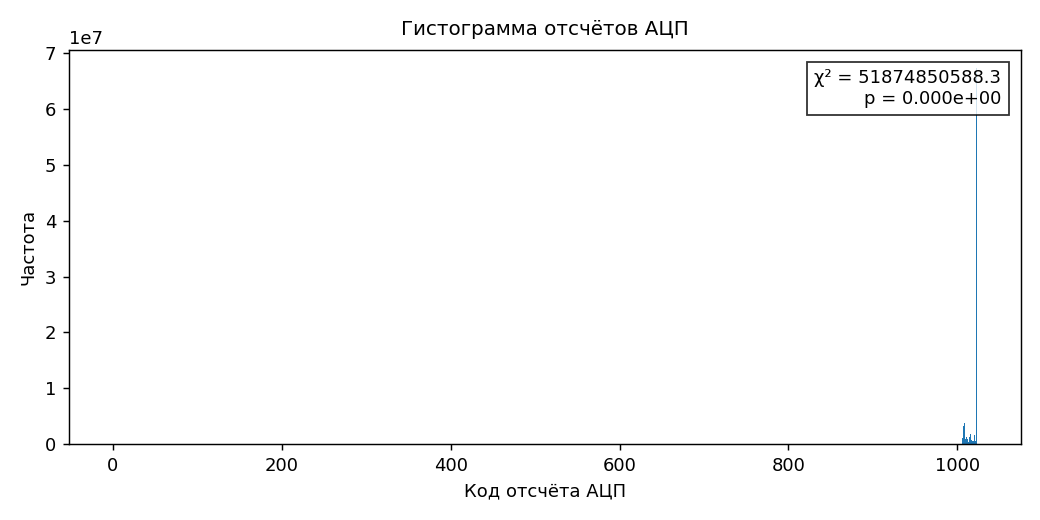
\includegraphics[width=\linewidth,keepaspectratio]{pandoc_media/media/exp_floating_adc/histogram_raw.png}
  \end{minipage}\hfill
  \begin{minipage}[t]{0.48\linewidth}
    \centering
    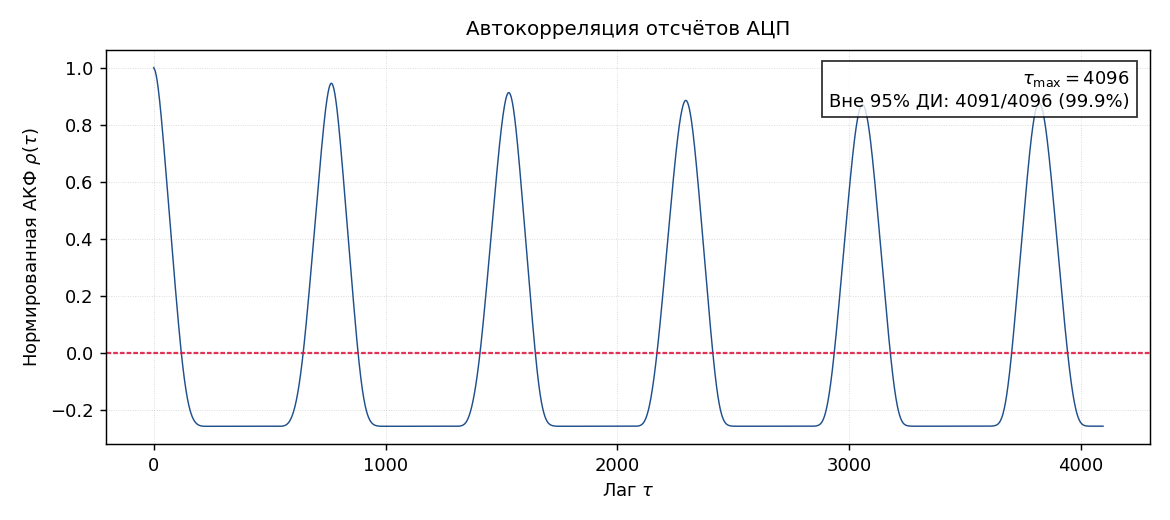
\includegraphics[width=\linewidth,keepaspectratio]{pandoc_media/media/exp_floating_adc/autocorr_raw.png}
  \end{minipage}
  \caption{Плавающий вход АЦП: гистограмма (концентрация в области $\sim 1020$) и
  автокорреляция отсчётов}
  \label{fig:floating_plots}
\end{figure}

Стандартное отклонение в шкале АЦП оказалось менее $6$ единиц, а среднее ---
непосредственно у верхнего предела шкалы ($1020$ из $1023$). Это означает, что
полезного <<шума>> на МЗР практически нет: значения почти всех отсчётов лежат
в крошечном окне $\sim 5$ единиц, и младший разряд жёстко связан со старшими.
Соответственно, NIST STS не проходит ни одной группы тестов даже после
постобработки фон Неймана; более того, эффективность фон Неймана здесь
катастрофически низкая (на выходе остаётся ${\approx} 6\%$ объёма входа),
что само по себе свидетельствует о сильной асимметрии исходного потока.

Раздел иллюстрирует широко распространённое заблуждение: типовой Arduino-код,
в котором затравка генератора инициализируется однократным чтением плавающего
аналогового входа --- \texttt{randomSeed(analogRead(A0))} --- а далее
<<случайные>> байты получаются вызовами \texttt{random(256)}, формально
проходит большинство тестов NIST STS. Это происходит потому, что алгоритм
\texttt{random()} в ядре Arduino --- линейный конгруэнтный генератор, и его
выход локально похож на равномерный. Однако каждая такая последовательность
\emph{полностью} определяется одним числом-затравкой (которое в данной
постановке несёт всего ${\sim}10$ бит исходной энтропии); зная алгоритм, всю
последующую <<случайную>> последовательность можно воспроизвести без
физического доступа к плате. Таким образом, для криптографических задач этот
шаблон опасен и должен быть отдельно оговорён в любых рекомендациях по
построению ГИСП на микроконтроллерах.

\crssubhead{3.8. MEMS-инерциальный датчик MPU-6050}

В качестве примера механического (точнее --- микроэлектромеханического) источника
энтропии исследовался шум показаний акселерометра/гироскопа MPU-6050, подключённого
к Arduino по шине I$^2$C. Микросхема MPU-6050 объединяет трёхосный акселерометр и
трёхосный гироскоп в общем корпусе; даже при неподвижном датчике в её показаниях
присутствует тепловой шум полупроводниковых преобразователей и собственно
механический шум подвижной массы. Для извлечения энтропии использовались
младшие разряды показаний всех шести осей; на каждый <<выходной байт>> приходилось
шесть бит от MPU-6050 и два дополнительных бита от соседних отсчётов АЦП для
дополнения до байта.

\begin{table}[H]
  \centering
  \footnotesize
  \caption{Параметры записи канала MPU-6050}
  \label{tab:mpu_summary}
  \begin{tabular}{|p{0.55\linewidth}|p{0.35\linewidth}|}
    \hline
    Число отсчётов & $\approx 5{,}2\cdot 10^6$ \\
    \hline
    Эффективная частота отсчётов $f_s$ & $\approx 700$~Гц \\
    \hline
    Среднее по шкале считанных байт & $31{,}5$ \\
    \hline
    Стандартное отклонение $\sigma$ & $18{,}5$ \\
    \hline
    Шеннон-энтропия на бит (выход прошивки) & $0{,}918$ \\
    \hline
    Минимальная энтропия на бит (MCV) & $0{,}584$ \\
    \hline
    NIST STS (LSB6): PASS / FAIL / N/A & $2$ / $11$ / $2$ \\
    \hline
  \end{tabular}
\end{table}

\begin{figure}[H]
  \centering
  \begin{minipage}[t]{0.48\linewidth}
    \centering
    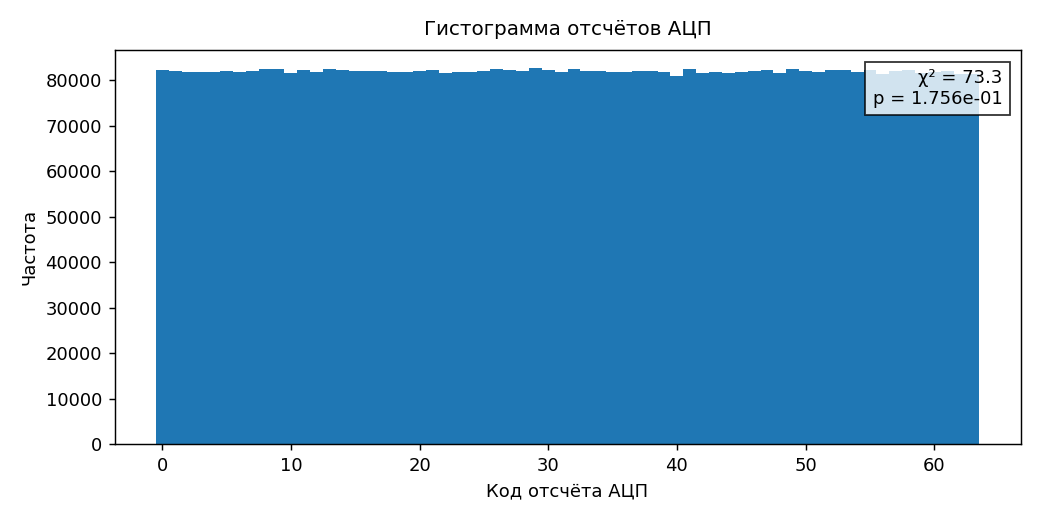
\includegraphics[width=\linewidth,keepaspectratio]{pandoc_media/media/exp_mpu6050/histogram_raw.png}
  \end{minipage}\hfill
  \begin{minipage}[t]{0.48\linewidth}
    \centering
    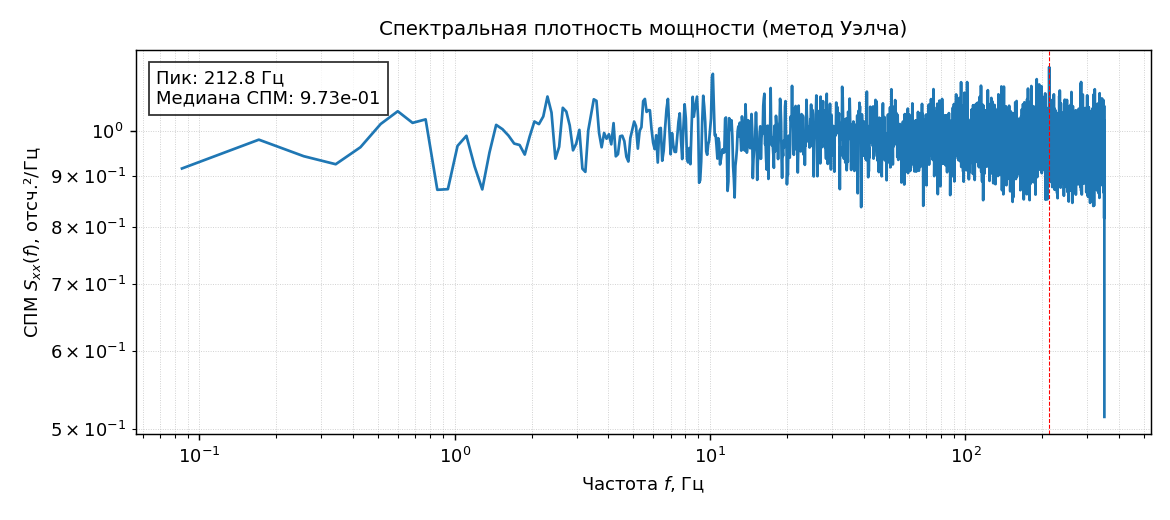
\includegraphics[width=\linewidth,keepaspectratio]{pandoc_media/media/exp_mpu6050/psd_raw.png}
  \end{minipage}
  \caption{MPU-6050: гистограмма выходных байтов и оценка спектральной плотности
  мощности}
  \label{fig:mpu_plots}
\end{figure}

MPU-6050 как источник энтропии страдает от двух принципиальных ограничений. Во-первых,
скорость генерации крайне низкая: реальная пропускная способность шины I$^2$C при
$400$~кГц и накладных расходах протокола ограничивает поток считываний значением
${\sim}10^3$ выборок в секунду, что на три порядка ниже, чем у аналоговых каналов.
Во-вторых, минимальная энтропия на бит ($0{,}58$) существенно ниже шенноновской
оценки ($0{,}92$), что говорит о выраженном смещении вероятности появления единиц
и нулей в одном из используемых разрядов. NIST STS даёт лишь $2$ PASS из $15$ ---
этого недостаточно даже для роли вспомогательного источника без существенного
усложнения постобработки.

Тем не менее, MPU-6050 сохраняет ценность в задачах формирования начального
состояния криптографических ГПСЧ (\textit{entropy seeding}) на этапе включения
устройства: даже несколько десятков байт с минимальной энтропией ${\sim}0{,}5$ бит
на бит позволяют гарантированно получить ${\sim}50\ldots 100$ бит энтропии за
несколько секунд, чего достаточно для инициализации типовых криптографических
ГПСЧ.

\crssubhead{3.9. Дрожание тактовых сигналов (clock jitter)}

В качестве чисто цифрового источника энтропии без аналоговой обвязки исследовался
относительный дрейф двух тактовых генераторов микроконтроллера ATmega328P: основного
кварцевого резонатора $16$~МГц и внутреннего RC-осциллятора сторожевого таймера
(\textit{watchdog timer}, WDT, ${\approx} 128$~кГц). В прошивке периодически
запускался короткий цикл WDT, и фиксировалось число тактов кварца, прошедшее
между двумя срабатываниями таймера. Младшие разряды этой разности отражают
относительную нестабильность RC-генератора относительно кварца --- фундаментально
случайный (тепловой и фазовый) процесс.

\begin{table}[H]
  \centering
  \footnotesize
  \caption{Параметры записи канала clock jitter}
  \label{tab:jitter_summary}
  \begin{tabular}{|p{0.55\linewidth}|p{0.35\linewidth}|}
    \hline
    Число отсчётов (uint16) & $864\,000$ \\
    \hline
    Эффективная частота отсчётов & $\approx 60$~Гц \\
    \hline
    Среднее по шкале счётчика & $32696$ \\
    \hline
    Стандартное отклонение $\sigma$ & $18919$ \\
    \hline
    Шеннон / минимальная энтропия на бит (LSB16) & $1{,}0000$ / $0{,}9997$ \\
    \hline
    NIST STS МЗР: PASS / FAIL / N/A & $1$ / $14$ / $0$ \\
    \hline
    NIST STS после VN (укороченный $3\times 10^6$~бит): PASS / FAIL / N/A & $0$ / $15$ / $0$ \\
    \hline
  \end{tabular}
\end{table}

\begin{figure}[H]
  \centering
  \begin{minipage}[t]{0.48\linewidth}
    \centering
    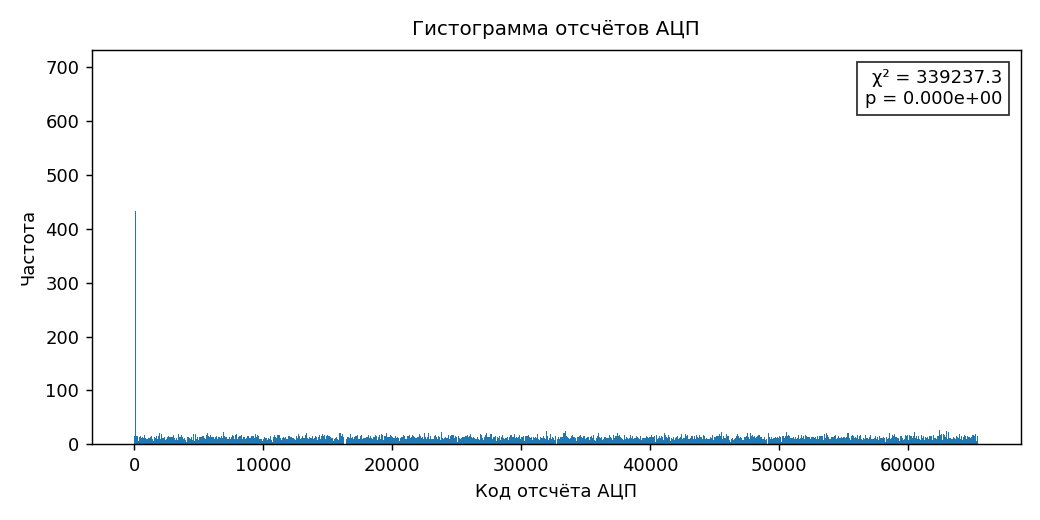
\includegraphics[width=\linewidth,keepaspectratio]{pandoc_media/media/exp_clock_jitter/histogram_raw.png}
  \end{minipage}\hfill
  \begin{minipage}[t]{0.48\linewidth}
    \centering
    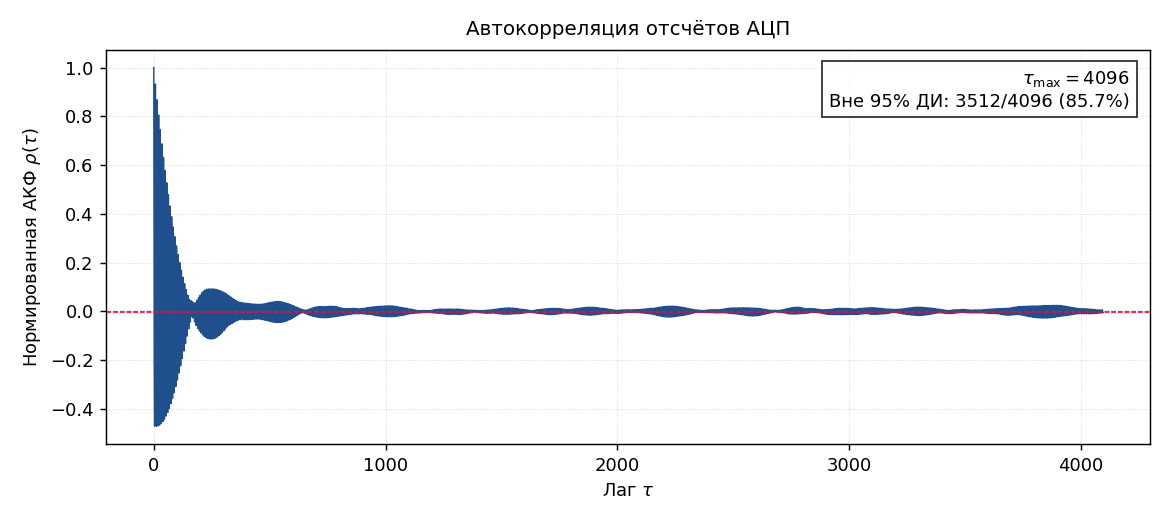
\includegraphics[width=\linewidth,keepaspectratio]{pandoc_media/media/exp_clock_jitter/autocorr_raw.png}
  \end{minipage}
  \caption{Канал clock jitter: гистограмма счётчика тактов и автокорреляция
  отсчётов}
  \label{fig:jitter_plots}
\end{figure}

Несмотря на формально высокие оценки энтропии на бит, ни МЗР, ни VN-выход не
проходят значимого количества тестов NIST. Причина в том, что MCU ATmega328P
имеет общий тактовый источник для большинства внутренних блоков, поэтому
эффективное число независимых источников фазового шума мало, и шумовая
составляющая в счётчике <<тонет>> в детерминированных временных
зависимостях. Кроме того, частота отсчётов ($\sim 60$~Гц) слишком низка для
накопления статистически значимого объёма данных за разумное время записи.

Тем не менее, канал clock jitter полезен в качестве <<нулевого по аппаратуре>>
вспомогательного источника энтропии в гибридных схемах: его можно фоном
накапливать без занятых аналоговых пинов и без увеличения BOM устройства.

\crssubhead{3.10. Итоги практической части и сравнение источников}

Сводные результаты шести исследованных в работе натурных каналов энтропии приведены в
таблице~\ref{tab:final_compare}. В качестве итогового критерия выбран профиль NIST
STS (PASS / FAIL / N/A) после постобработки фон Неймана, дополненный показателями
скорости генерации (битов в секунду на выходе VN) и минимальной энтропии на бит.

\begin{table}[H]
  \centering
  \footnotesize
  \caption{Сравнительная характеристика натурных источников энтропии,
  исследованных в работе. NIST STS приведён для последовательности после
  постобработки фон Неймана}
  \label{tab:final_compare}
  \begin{tabular}{|p{0.22\linewidth}|p{0.16\linewidth}|p{0.10\linewidth}|p{0.13\linewidth}|p{0.10\linewidth}|p{0.13\linewidth}|}
    \hline
    Источник & Сложность аппаратуры & $\sigma$ АЦП & NIST PASS / FAIL & min-H (бит) & Скорость VN, бит/с \\
    \hline
    BJT (этап~4) + VN + \texttt{decim\_xor8win} & низкая (1~ОУ, 1~BJT) & $146{,}5$ & \textbf{15 / 0} & $0{,}9999$ & ${\sim} 1{,}6\cdot 10^3$ \\
    \hline
    BJT (этап~4) + VN (базовый) & низкая (1~ОУ, 1~BJT) & $146{,}5$ & 13 / 2 & $0{,}9999$ & ${\sim} 1{,}3\cdot 10^4$ \\
    \hline
    Тепловой шум $10$~МОм & низкая (1~ОУ) & $14{,}6$ & 10 / 5 & $0{,}9984$ & ${\sim} 1{,}5\cdot 10^4$ \\
    \hline
    Микрофон KY-037 & низкая (готовый модуль) & $0{,}90$ & 4 / 11 & $0{,}9994$ & ${\sim} 7{,}5\cdot 10^3$ \\
    \hline
    MPU-6050 (MEMS) & средняя (модуль I$^2$C) & --- & 2 / 11 & $0{,}584$ & ${\sim} 5{,}6\cdot 10^3$ \\
    \hline
    Clock jitter (WDT) & минимальная (только MCU) & --- & 0 / 15 (VN) / 1 / 14 (LSB) & $0{,}9997$ & ${\sim} 30$ \\
    \hline
    Плавающий ADC & минимальная (только MCU) & $5{,}3$ & 0 / 15 (VN) & $0{,}9994$ & ${\sim} 200$ \\
    \hline
  \end{tabular}
\end{table}

Среди натурно проверенных каналов наилучший результат как по формальному профилю
NIST STS, так и по физической форме полезного сигнала достигнут источником
\textbf{лавинного шума BE-перехода BJT} в итоговой конфигурации (этап~4
раздела~3.5) с \emph{двухступенчатой} постобработкой по схеме фон Нейман $\to$
\texttt{decim\_xor8win} (раздел~3.5.8): полный профиль \textbf{$15$ PASS из $15$}
групп тестов NIST STS, минимальная энтропия на бит $0{,}9999$, скорость выхода
после каскадной постобработки $\sim 1{,}6$~кбит/с и стоимость элементной базы
менее $50$~рублей. Это означает, что построенный из дешёвых компонентов и без
криптографических библиотек источник по статистике совпадает с эталонной случайной
последовательностью. Базовая конфигурация без второго прохода (только фон Нейман,
$13$ PASS из $15$) сохраняет ценность как компромисс по скорости: при $10$~кбит/с
она почти на порядок быстрее каскадной и достаточна для подавляющего большинства
прикладных задач, где допустимы остаточные провалы в группах тестов случайных
блужданий. Основные направления дальнейшего развития (раздел~3.11): интеграция
второго аналогичного канала на втором канале сдвоенного ОУ с XOR-смешением,
переход на печатную плату с улучшенным экранированием и упаковка стенда в
законченный модуль с собственным микроконтроллером.

Тепловой канал на резисторе $10$~МОм после исправления методики измерения
демонстрирует устойчивый <<средний>> результат ($10$ PASS из $15$) при сопоставимой
скорости генерации, однако амплитуда полезного сигнала на порядок ниже, чем у
лавинного источника, что повышает требования к точности усилителя и развязке
по питанию. Акустический канал на готовом микрофонном модуле KY-037 в типичной
бытовой обстановке оказался неспособен использовать динамический диапазон АЦП
($\sigma_\mathrm{adc}<1$) и сохранил выраженную узкополосную компоненту
${\approx}371$~Гц --- даже после фон Неймана из NIST STS проходят всего
$4$ группы тестов. MPU-6050 как самостоятельный источник существенно слабее,
но может выполнять роль вспомогательного канала для инициализации начального
состояния криптографических ГПСЧ в гибридных схемах. Плавающий вход АЦП и
замер дрожания тактовых сигналов (clock jitter), несмотря на формально высокие
бит-энтропийные оценки, в наблюдаемой реализации непригодны для использования
в роли самостоятельных источников и приводятся в работе скорее как иллюстрация
типичных заблуждений начинающих разработчиков.

Главный методический вывод раздела состоит в следующем: при разработке
аппаратного ГИСП оценка качества источника не сводится к формальному прогону
NIST STS на МЗР --- необходимо комплексное обследование физической формы сигнала
(гистограмма, насыщение, узкополосные компоненты), осознанная работа с
динамическим диапазоном усилителя и АЦП, проверка устойчивости конфигурации к
варьируемым внешним условиям (питание, нагрев) и, наконец, использование
постобработки, обоснованной для конкретного типа смещения исходного потока.
Совмещение всех четырёх требований и стало основой описанной в разделе~3.5
методики работы с каналом BJT.

\crssubhead{3.11. Перспективные направления развития физических генераторов случайных последовательностей (ФГСП)}

Современные требования к безопасности информационных систем, а также
рост применения криптографических и статистических методов в различных
областях обуславливают необходимость дальнейшего совершенствования
физических генераторов случайных последовательностей (ФГСП). Развитие
данных систем направлено на повышение их надёжности, устойчивости к
внешним воздействиям, скорости генерации и интеграции в современные
аппаратные платформы. Ниже рассмотрены ключевые направления развития.

Миниатюризация и интеграция в чипы. Современные технологии производства
микросхем позволяют встраивать элементы ФГСП непосредственно в
процессоры, контроллеры и криптографические сопроцессоры. Это
обеспечивает минимальные задержки при получении случайных битов и
упрощает защиту от атак на уровне интерфейсов. Развитие технологии CMOS,
FinFET и перспективных материалов способствует созданию компактных,
энергоэффективных и массовых решений.

Перспективным направлением является использование квантовых источников
энтропии --- в частности, спонтанного распада фотонов, квантовых
флуктуаций вакуума и эффекта туннелирования. Такие источники обладают
высокой степенью истинной случайности, подтверждаемой теорией квантовой
неопределённости, и демонстрируют устойчивость к предсказуемости со
стороны атакующего. Разработка доступных и стабильно работающих
квантовых ФГСП, увеличение скорости их генерации остаются важной
задачей.

Оптические и фотонные источники также могут быть подвержены
модернизации. Оптические ФГСП, основанные на фотоэлектрическом шуме,
колебаниях интенсивности лазерного излучения и спонтанном рассеянии
света, демонстрируют высокую пропускную способность и низкую
коррелированность выходных битов. Развитие интегральной фотоники и
кремниевых фотонных чипов позволяет создавать компактные и
масштабируемые оптические генераторы с высокой скоростью и надёжностью.

Повышение надёжности генерации достигается за счёт объединения
нескольких физических источников энтропии в гибридной архитектуре.
Комбинация теплового, дробового, лавинного шумов, а также оптических и
квантовых источников позволяет компенсировать слабости отдельных
компонентов, а также реализовать адаптивные схемы оценки качества и
селекции наиболее надёжных источников в реальном времени. Таким образом,
перспективным направлением развития является изучение комбинаций
источников энтропии в ФГСП: многоканальные и гибридные схемы.

Совершенствование методов постобработки, внедрение постобработки на
аппаратном уровне также являются современной тенденцией развития ФГСП.
Для повышения энтропийной насыщенности и устранения смещения (bias)
усиливается внимание к аппаратной реализации алгоритмов экстракции,
таких как схема фон Неймана, хэш-функции и решёточные методы. Аппаратная
реализация постобработки позволяет достичь высокой скорости и
энергоэффективности без ущерба для статистических свойств выходных
данных.

Современные подходы к верификации и мониторингу работы ФГСП
предусматривают встраивание модулей контроля, способных выполнять
непрерывное статистическое тестирование и выявление деградации качества
энтропии. Это особенно важно в критических приложениях, где отклонения в
характеристиках могут привести к серьёзным уязвимостям. С появлением
новых способов атаки на ФГСП также появляется необходимость в
поддержании эффективного автоматического тестирования и самодиагностики.

В рамках международных инициатив (например, NIST, ISO) разрабатываются
единые подходы к оценке качества ФГСП. Это способствует унификации
требований, повышению доверия к устройствам и упрощению их внедрения в
сертифицированные системы безопасности.

В совокупности данные направления определяют вектор дальнейших
исследований и разработок в области ФГСП, ориентируясь на создание
высоконадёжных, воспроизводимых и проверяемых источников истинной
случайности для современных и перспективных информационно-технических
систем.
